% =====================================================================
%  Rapport technique – Mini-projet Systèmes Intégrés (INSEA, 2026-2027)
%  Module Odoo 19 « Congés & Absences » (insea_hr_leave_custom)
%  Compilation : latexmk -pdf rapport.tex   (ou pdflatex x2)
% =====================================================================
\documentclass[11pt,a4paper]{article}

% ---------------------------------------------------------------------
% Informations de la page de garde
% ---------------------------------------------------------------------
\newcommand{\auteurs}{KADADE MAHAMADOU Bassirou}
\newcommand{\encadrant}{Pr. OURADI Najib}
\newcommand{\master}{Système d'Information et Système Intelligent (M2SI)}
\newcommand{\niveau}{2\textsuperscript{e} année}
\newcommand{\annee}{2026--2027}

% ---------------------------------------------------------------------
\usepackage[utf8]{inputenc}
\usepackage[T1]{fontenc}
\usepackage[french]{babel}
\usepackage{lmodern}
\usepackage{microtype}
\usepackage[a4paper,margin=2.2cm,top=2.3cm,bottom=2.4cm]{geometry}
\usepackage{graphicx}
\usepackage{float}
\usepackage{booktabs}
\usepackage{tabularx}
\usepackage{array}
\usepackage{longtable}
\usepackage[table]{xcolor}
\usepackage{enumitem}
\usepackage{caption}
\usepackage{subcaption}
\usepackage{fancyhdr}
\usepackage{titlesec}
\usepackage{listings}
\usepackage{amssymb}
\usepackage{tikz}
\usetikzlibrary{arrows.meta}
\usepackage{hyperref}

\definecolor{inseagreen}{RGB}{0,128,90}
\definecolor{codebg}{RGB}{246,248,250}
\definecolor{codegray}{RGB}{110,110,110}

\newcommand{\repourl}{https://github.com/BassirouKadade/odoo-conges-absences}
\hypersetup{
  colorlinks=true, linkcolor=black, citecolor=black, urlcolor=inseagreen,
  pdftitle={Congés \& Absences - Module Odoo 19},
  pdfauthor={INSEA - M2SI},
  pdfsubject={Mini-projet Systèmes Intégrés},
}

\captionsetup{font=small,labelfont=bf,labelsep=colon}
\setlength{\parskip}{4pt}
\setlength{\parindent}{0pt}
\setlist{itemsep=2pt,topsep=3pt}
\renewcommand{\arraystretch}{1.18}
\newcolumntype{Y}{>{\raggedright\arraybackslash}X}

\titleformat{\section}{\Large\bfseries\color{inseagreen}}{\thesection}{0.8em}{}
\titleformat{\subsection}{\large\bfseries}{\thesubsection}{0.8em}{}
\titleformat{\subsubsection}{\normalsize\bfseries}{\thesubsubsection}{0.8em}{}

\pagestyle{fancy}
\fancyhf{}
\fancyhead[L]{\small\color{codegray}Congés \& Absences -- Module Odoo 19}
\fancyhead[R]{\small\color{codegray}Systèmes Intégrés -- INSEA}
\fancyfoot[C]{\small Page \thepage}
\renewcommand{\headrulewidth}{0.3pt}

\newcommand{\code}[1]{\texttt{\detokenize{#1}}}
\newcommand{\fig}[3][\textwidth]{%
  \begin{figure}[H]\centering\includegraphics[width=#1]{#2}\caption{#3}\end{figure}}

\lstset{
  basicstyle=\ttfamily\footnotesize,
  backgroundcolor=\color{codebg},
  frame=single, rulecolor=\color{black!15},
  breaklines=true, columns=fullflexible,
  keywordstyle=\color{inseagreen}\bfseries,
  commentstyle=\color{codegray}\itshape,
  stringstyle=\color{black!70},
  showstringspaces=false,
  xleftmargin=4pt, xrightmargin=4pt,
  literate={é}{{\'e}}1 {è}{{\`e}}1 {à}{{\`a}}1 {ç}{{\c{c}}}1 {ê}{{\^e}}1 {É}{{\'E}}1
           {ô}{{\^o}}1 {î}{{\^i}}1 {ù}{{\`u}}1 {â}{{\^a}}1 {û}{{\^u}}1 {ï}{{\"i}}1 {ë}{{\"e}}1
           {À}{{\`A}}1 {Ç}{{\c{C}}}1 {È}{{\`E}}1 {Ê}{{\^E}}1
           {→}{{$\rightarrow$}}1 {≤}{{$\leq$}}1 {≥}{{$\geq$}}1,
}

\begin{document}

% =====================================================================
% PAGE DE GARDE
% =====================================================================
\begin{titlepage}
\newgeometry{margin=1.8cm,top=1.4cm,bottom=1.8cm}
\centering
% ----- En-tête institutionnel : HCP | Royaume du Maroc / HCP / INSEA | INSEA -----
\begin{minipage}[c]{0.27\textwidth}
  \raggedright
  
\includegraphics[width=3.9cm]{img/logo_hcp.png}
\end{minipage}%
\begin{minipage}[c]{0.46\textwidth}
  \centering
  {\small\scshape Royaume du Maroc}\\[1pt]
  {\scriptsize $\ast\ast\ast\ast\ast$}\\[1pt]
  {\small\scshape Haut Commissariat au Plan}\\[1pt]
  {\scriptsize $\ast\ast\ast\ast\ast$}\\[2pt]
  {\small\bfseries\scshape Institut National de Statistique\\ et d'Économie Appliquée}
\end{minipage}%
\begin{minipage}[c]{0.27\textwidth}
  \raggedleft
  
\includegraphics[width=2.2cm]{img/logo_insea.png}
\end{minipage}

\vspace*{\stretch{1.1}}

% ----- Icône de l'application (annotée), puis titre -----
\begin{tikzpicture}
  \node[inner sep=0] (logo) at (0,0) {
\includegraphics[width=2.1cm]{img/app_icon.png}};
  % étiquette et flèche en « overlay » : le logo reste centré sur la page
  \node[overlay, anchor=east, align=right, text=black!65, font=\small\itshape] (lbl) at (-3.1,1.05)
       {Logo du module Odoo\\ « Congés \& Absences »,\\ conçu pour ce projet};
  \draw[overlay, black!40, line width=1.3pt, line cap=round, -{Stealth[length=3.2mm,width=2.8mm]}]
       plot[smooth, tension=0.75] coordinates
       {(-3.0,0.95) (-2.55,0.75) (-2.2,0.3) (-2.45,-0.05) (-2.75,0.2) (-2.45,0.45) (-2.05,0.05) (-1.35,-0.05)};
\end{tikzpicture}\\[0.6cm]
{\large\scshape Rapport technique du mini-projet}\\[0.55cm]
{\color{inseagreen}\rule{0.55\linewidth}{0.6pt}}\\[0.5cm]
{\fontsize{34}{40}\selectfont\bfseries\color{inseagreen} Congés \& Absences}\\[0.45cm]
{\Large\bfseries Module Odoo de gestion des autorisations\\[3pt] d'absence et des congés}\\[0.45cm]
{\large\itshape Conception UML, développement Odoo~19 et validation}\\[0.5cm]
{\color{inseagreen}\rule{0.55\linewidth}{0.6pt}}

\vspace*{\stretch{0.7}}

% ----- Cadre académique -----
{\small Projet réalisé dans le cadre du module}\\[3pt]
{\Large\bfseries SYSTÈMES INTÉGRÉS}

\vspace*{\stretch{1.4}}

% ----- Auteur et encadrant (seuls en bas de page) -----
\begin{minipage}[t]{0.46\textwidth}
\raggedright
{\small\color{inseagreen}\bfseries RÉALISÉ PAR}\\[3pt]
{\large \auteurs}\\[6pt]
{\small Filière : \textbf{M2SI}}\\[2pt]
{\small Année universitaire : \textbf{\annee}}
\end{minipage}\hfill
\begin{minipage}[t]{0.46\textwidth}
\raggedleft
{\small\color{inseagreen}\bfseries ENCADRÉ PAR}\\[3pt]
{\large \encadrant}
\end{minipage}
\restoregeometry
\end{titlepage}

% =====================================================================
\tableofcontents
\newpage

% =====================================================================
\section{Introduction}
% =====================================================================

\subsection{Contexte et problématique}
La société Lambda gère aujourd'hui ses absences de courte durée et ses congés légaux à l'aide de
formulaires papier et d'échanges informels. Le cahier des charges du mini-projet relève trois
conséquences : des retards de validation, des erreurs dans le décompte du solde de congés payés et
une visibilité insuffisante des managers lors de la planification des équipes.

L'objectif est de dématérialiser ce circuit dans l'ERP open source \textbf{Odoo}, au moyen d'un
module dédié. Le module réalisé, \code{insea_hr_leave_custom}, est publié dans Odoo sous le nom
\textbf{« Congés \& Absences »}.

\subsection{Objectifs et périmètre}
Le module couvre les deux volets du cahier des charges :
\begin{itemize}
  \item \textbf{les autorisations de sortie} : absences de quelques heures (4~h au maximum), soumises
        à un plafond mensuel et à un motif obligatoire ;
  \item \textbf{les congés légaux} : congé payé annuel, congé exceptionnel pour événement familial et
        congé maladie.
\end{itemize}
Chaque demande suit un circuit de validation à deux niveaux (manager N+1, puis Responsable RH),
contrôlé par une machine à états et par les groupes de sécurité d'Odoo.

\subsection{Démarche et organisation du rapport}
Nous avons suivi une démarche classique : expression des besoins, conception UML, développement,
puis validation par des tests automatisés et un jeu de données de démonstration. Le rapport suit
le même ordre. La section~\ref{sec:besoins} reformule les besoins. La section~\ref{sec:uml}
présente les modèles UML. La section~\ref{sec:archi} décrit l'architecture technique et la
section~\ref{sec:impl} les choix d'implémentation dans Odoo. Les interfaces sont présentées en
section~\ref{sec:ihm}, les tests en section~\ref{sec:tests}. Nous terminons par les limites
connues et les perspectives.

% =====================================================================
\section{Expression des besoins}\label{sec:besoins}
% =====================================================================

\subsection{Acteurs du système}
Le cahier des charges impose quatre rôles. Nous ajoutons un acteur secondaire non humain, le
système lui-même, qui exécute les traitements automatiques. Le rôle d'\emph{administrateur
fonctionnel} (paramétrage des types de congés, motifs et règles) est confié au Responsable RH ;
l'Administrateur système garde l'installation et la gestion technique des comptes.

\begin{table}[H]
\centering
\caption{Acteurs, responsabilités et périmètre de visibilité.}
\label{tab:acteurs}
\small
\begin{tabularx}{\textwidth}{>{\bfseries}l Y l}
\toprule
Acteur & Responsabilités & Visibilité des demandes \\
\midrule
Employé & Crée, justifie et soumet ses demandes ; consulte son solde. & Les siennes \\
Manager (N+1) & Approuve ou refuse les demandes de son équipe ; son approbation est finale
pour une autorisation de sortie. & Son équipe \\
Responsable RH & Seconde validation des congés, vérification des justificatifs, gestion des soldes,
paramétrage (administrateur fonctionnel). & Toutes \\
Administrateur système & Installe le module, gère les utilisateurs, les groupes et la hiérarchie. &
Configuration \\
Système (cron) & Crédite 1,5~jour par mois, exécute les contrôles, envoie les notifications. &
-- \\
\bottomrule
\end{tabularx}
\end{table}

Le Manager et le Responsable RH sont aussi des employés : ils posent eux-mêmes des demandes. Cette
relation est modélisée par une généralisation dans le diagramme de cas d'utilisation et par
l'héritage des groupes de sécurité (section~\ref{sec:securite}).

\subsection{Règles de gestion}
Le tableau~\ref{tab:regles} reprend les règles du cahier des charges et indique, pour chacune,
le moment où le module la vérifie.

\begin{table}[H]
\centering
\caption{Règles de gestion du cahier des charges et moment du contrôle.}
\label{tab:regles}
\small
\begin{tabularx}{\textwidth}{>{\raggedright\arraybackslash}p{4.3cm} Y l}
\toprule
Règle & Énoncé & Contrôle \\
\midrule
Durée d'une sortie & Au plus 4~heures, le même jour. & Enregistrement \\
Plafond mensuel des sorties & Au plus 3 autorisations \emph{ou} 8~heures cumulées par mois
calendaire. & Soumission \\
Non-chevauchement & Aucune demande ne peut recouvrir une demande du même collaborateur déjà
soumise, en validation ou approuvée. & Enregistrement \\
Solde de congés payés & Le solde disponible (acquis à 1,5~jour par mois) doit être supérieur ou
égal à la durée demandée. & Soumission \\
Délai de prévenance & Un congé payé de plus de 3~jours est soumis au moins 7~jours calendaires à
l'avance. & Soumission \\
Congés exceptionnels & Mariage : 4~jours ; naissance : 3~jours ; décès : 2 à 3~jours. &
Enregistrement \\
Justificatif & Obligatoire pour la maladie, les événements familiaux et la sortie pour motif
médical ; il bloque la validation finale. & Validation RH \\
Impact sur le solde & Seul le congé payé annuel est déduit du solde ; la sortie ne l'est pas. &
Validation RH \\
\bottomrule
\end{tabularx}
\end{table}

\subsection{Exigences non fonctionnelles}
\begin{itemize}
  \item \textbf{Sécurité} : un employé ne consulte que ses demandes, un manager celles de son équipe,
        le RH l'ensemble (règles d'enregistrement).
  \item \textbf{Traçabilité} : chaque changement d'état et chaque décision est historisé (chatter
        Odoo, champs de suivi des valideurs).
  \item \textbf{Ergonomie} : les boutons d'action ne s'affichent qu'à la personne habilitée ; les
        messages d'erreur sont rédigés en français et indiquent la valeur en cause.
  \item \textbf{Isolation de l'environnement} : la pile Docker du projet ne doit pas entrer en
        collision avec un autre projet Odoo présent sur la même machine.
\end{itemize}

% =====================================================================
\section{Conception UML}\label{sec:uml}
% =====================================================================
Les diagrammes ont été réalisés avec PlantUML ; leurs sources se trouvent dans \code{docs/uml/}.

\subsection{Diagrammes de cas d'utilisation}
Un diagramme unique regroupant tous les cas d'utilisation était illisible. Nous l'avons découpé en
une vue d'ensemble (figure~\ref{fig:uc0}) et trois diagrammes détaillés.

\begin{figure}[H]
\centering
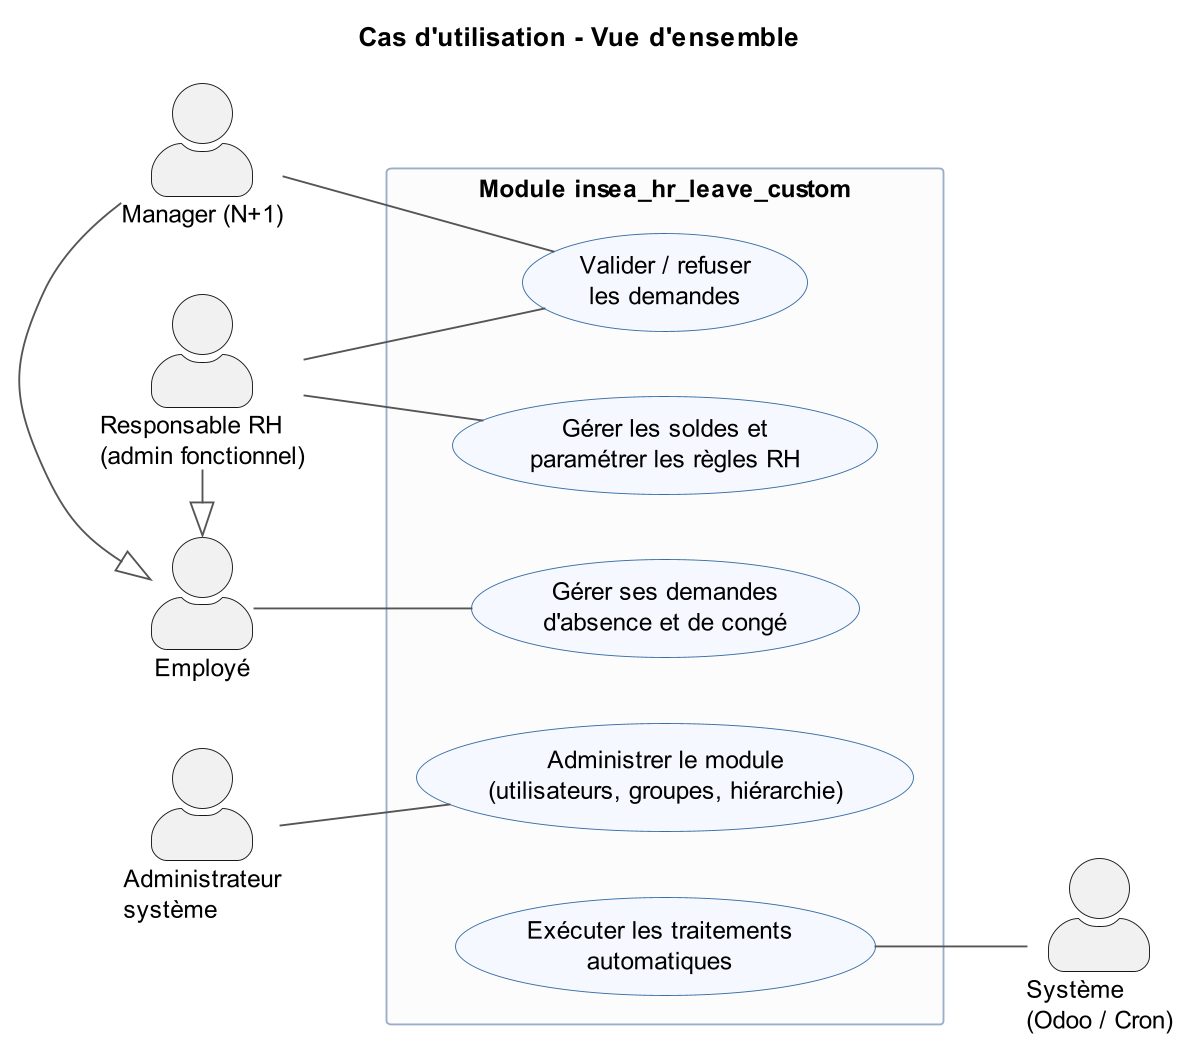
\includegraphics[width=0.78\textwidth]{img/uml/uc_0_vue_ensemble.png}
\caption{Vue d'ensemble : les cinq acteurs et les cinq domaines fonctionnels. Le Manager et le
Responsable RH spécialisent l'Employé.}
\label{fig:uc0}
\end{figure}

\begin{figure}[H]
\centering
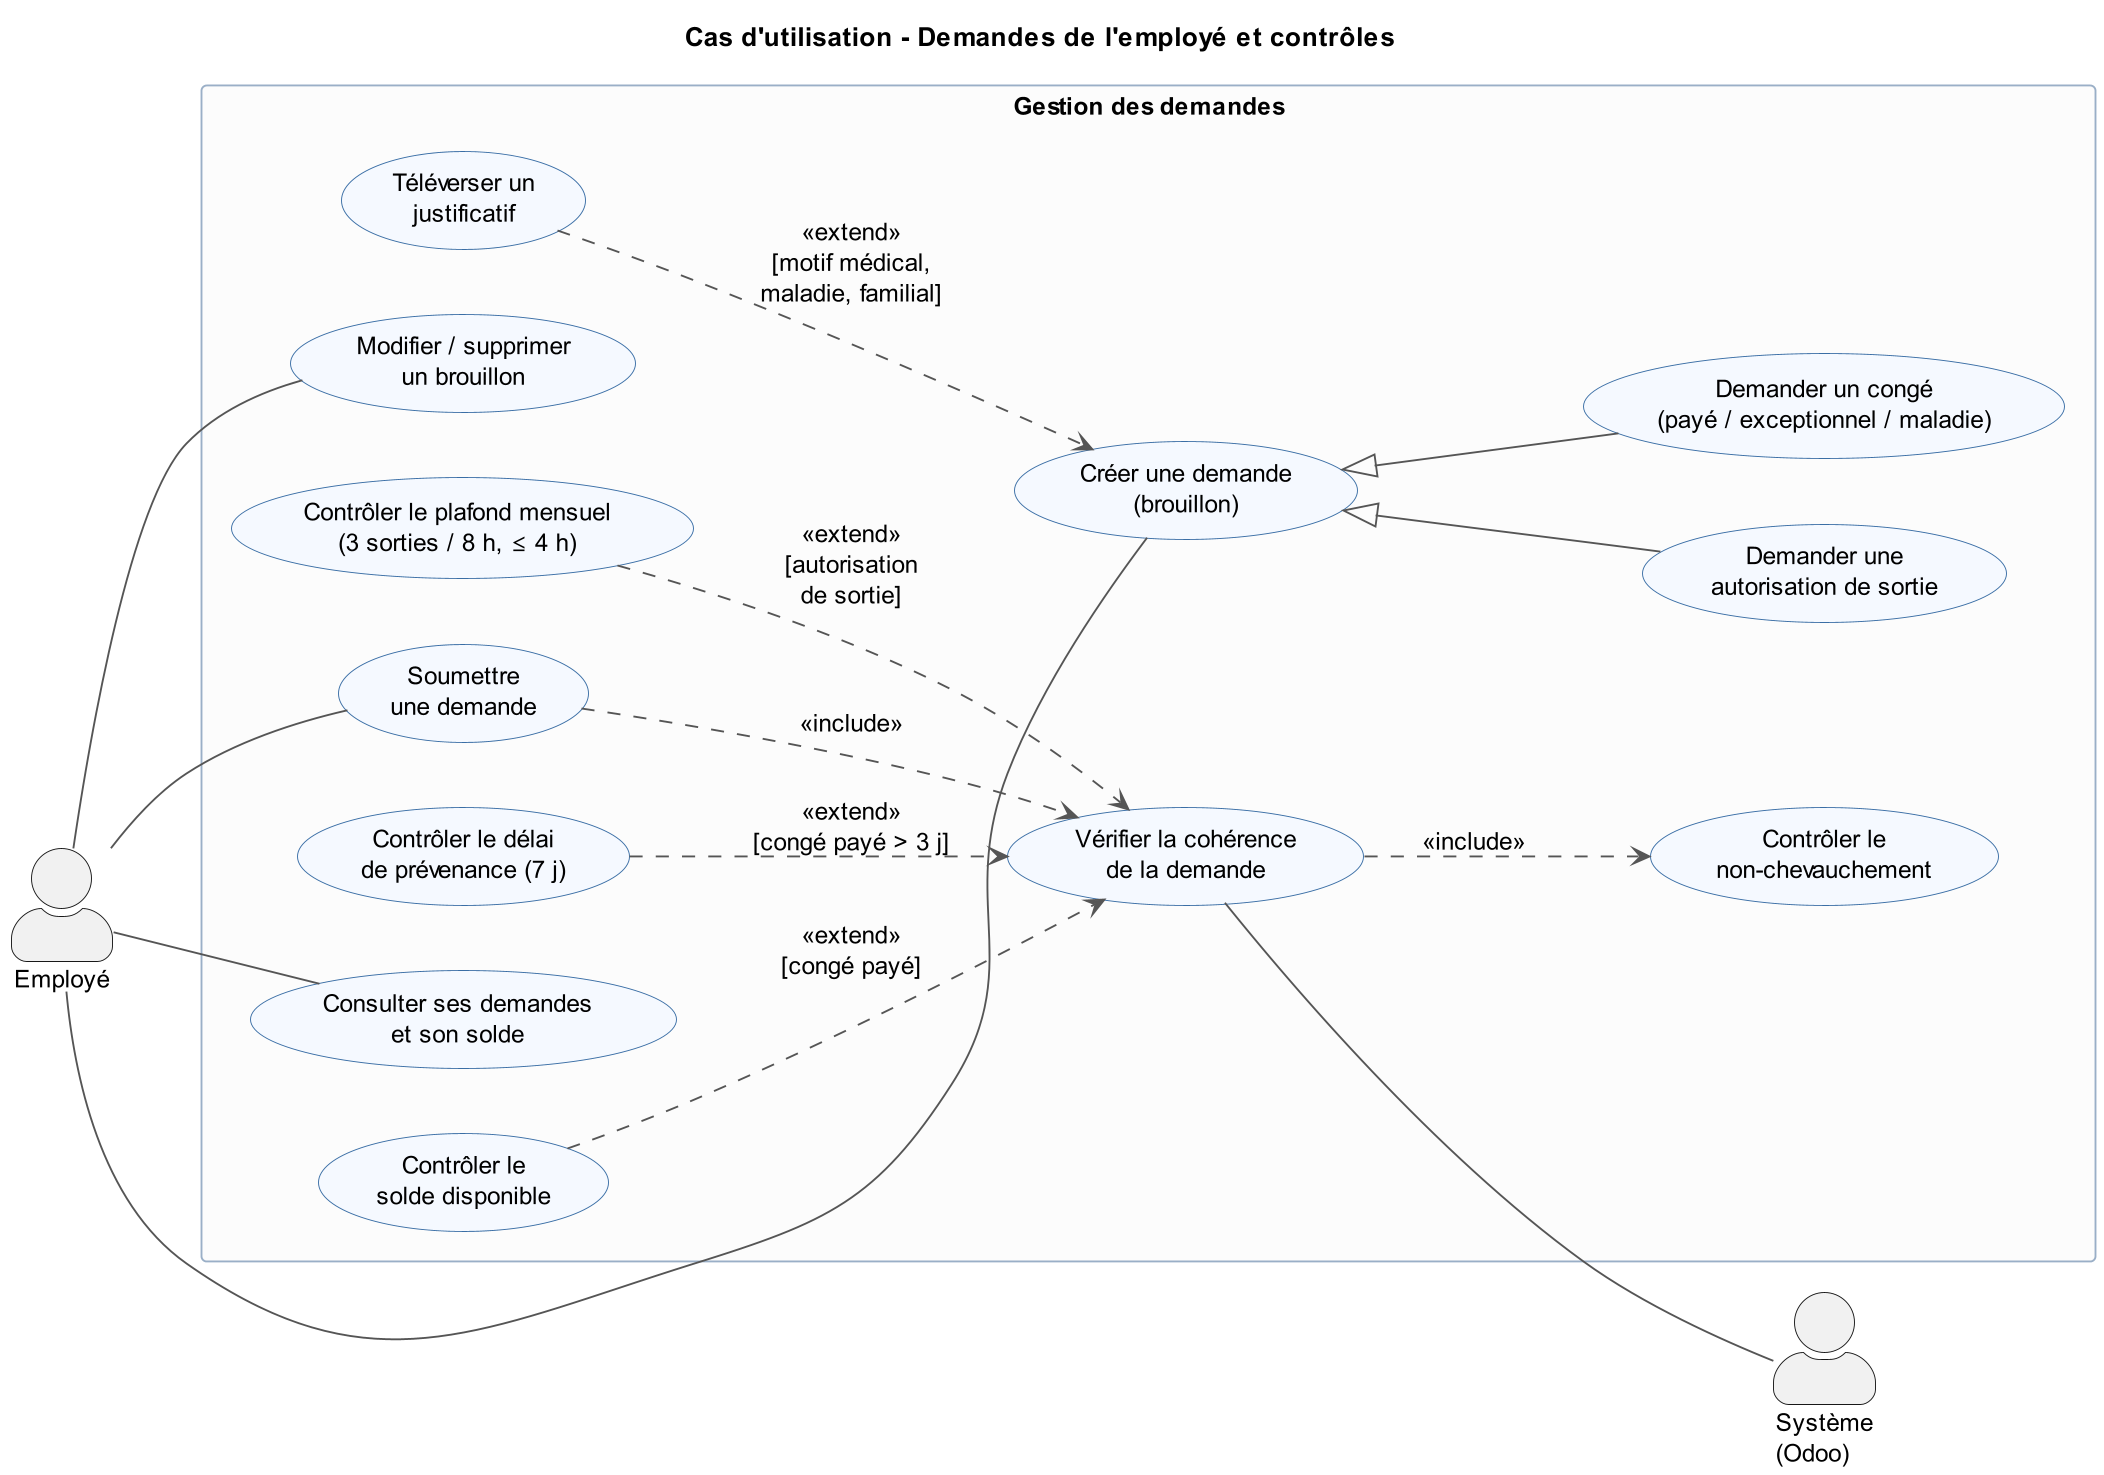
\includegraphics[width=\textwidth]{img/uml/uc_1_demandes.png}
\caption{Demandes de l'employé et contrôles. La soumission \emph{inclut} la vérification de cohérence,
qui inclut toujours le non-chevauchement ; les contrôles du solde, du délai et du plafond
\emph{étendent} cette vérification selon le type de demande.}
\label{fig:uc1}
\end{figure}

\begin{figure}[H]
\centering
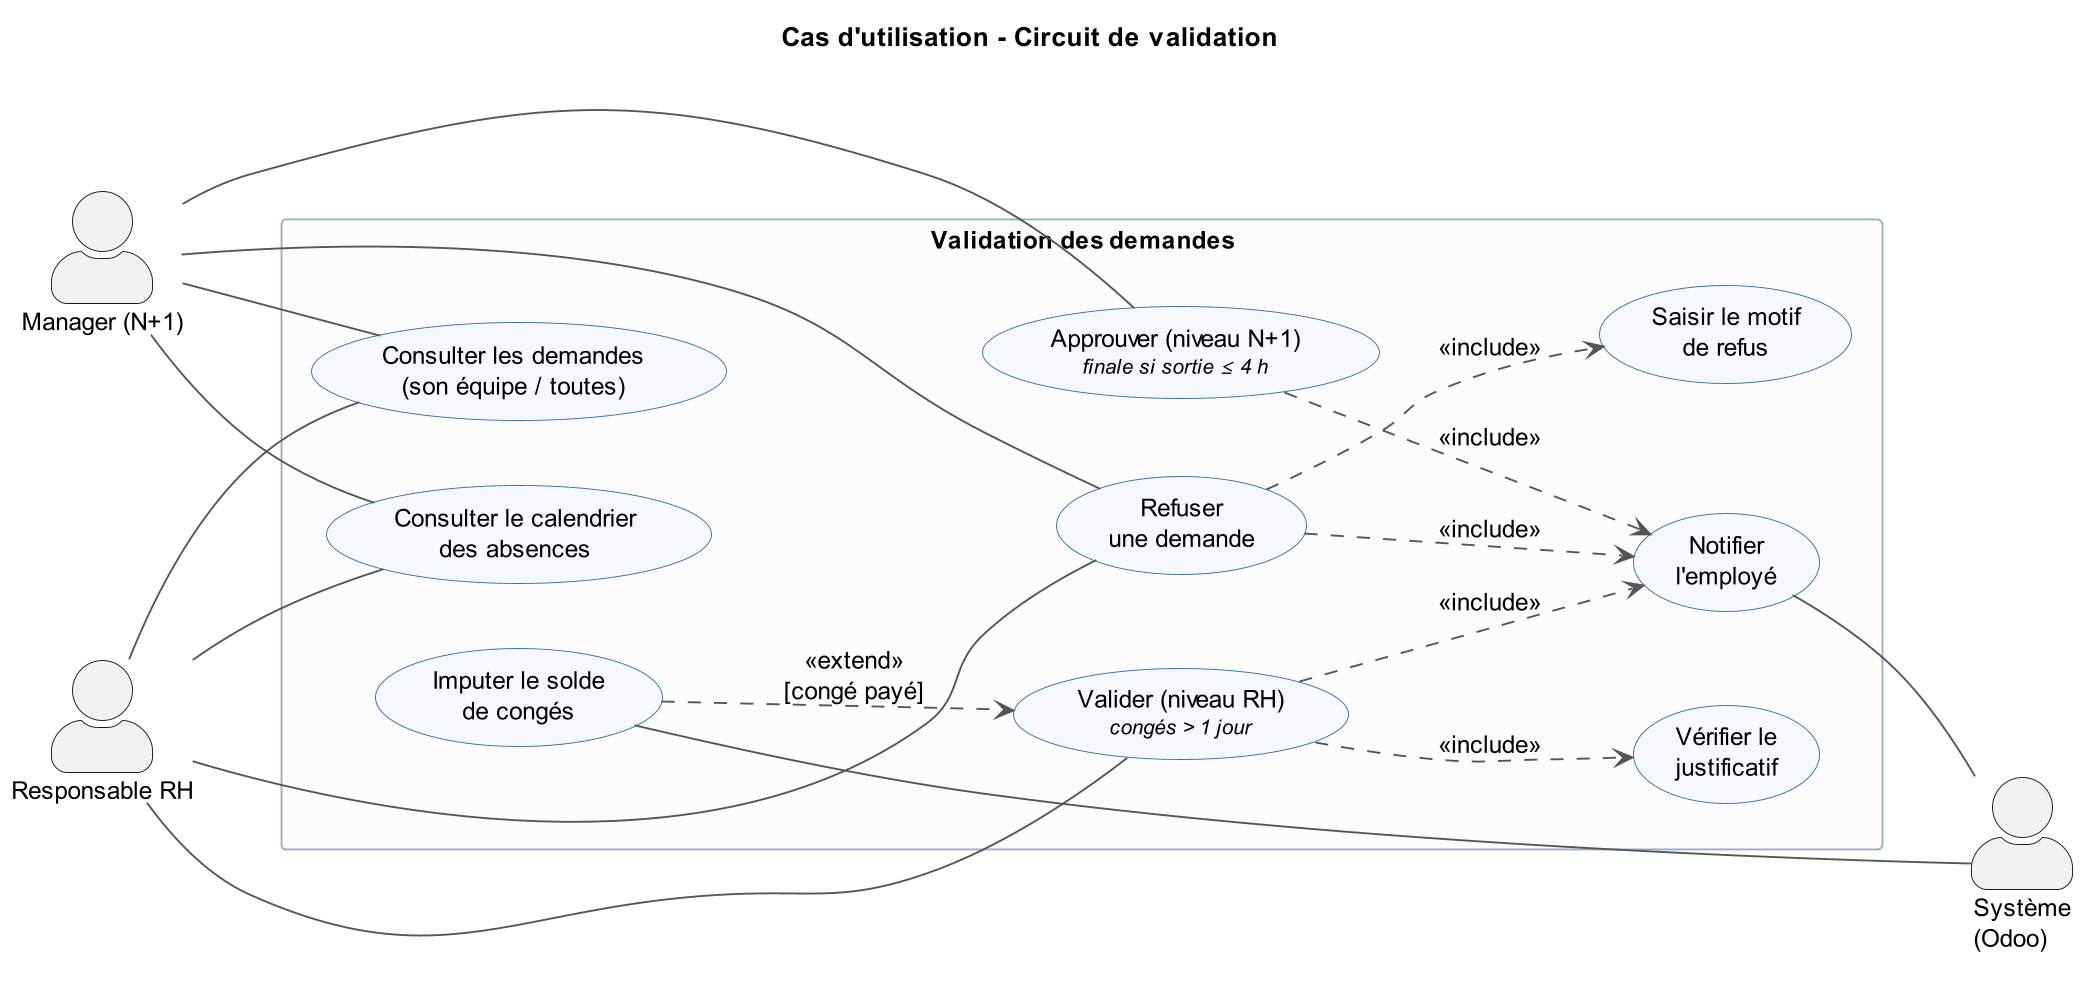
\includegraphics[width=\textwidth]{img/uml/uc_2_validation.png}
\caption{Circuit de validation. Le refus inclut la saisie du motif et la notification de l'employé ;
l'imputation du solde étend la validation RH pour le congé payé.}
\label{fig:uc2}
\end{figure}

\begin{figure}[H]
\centering
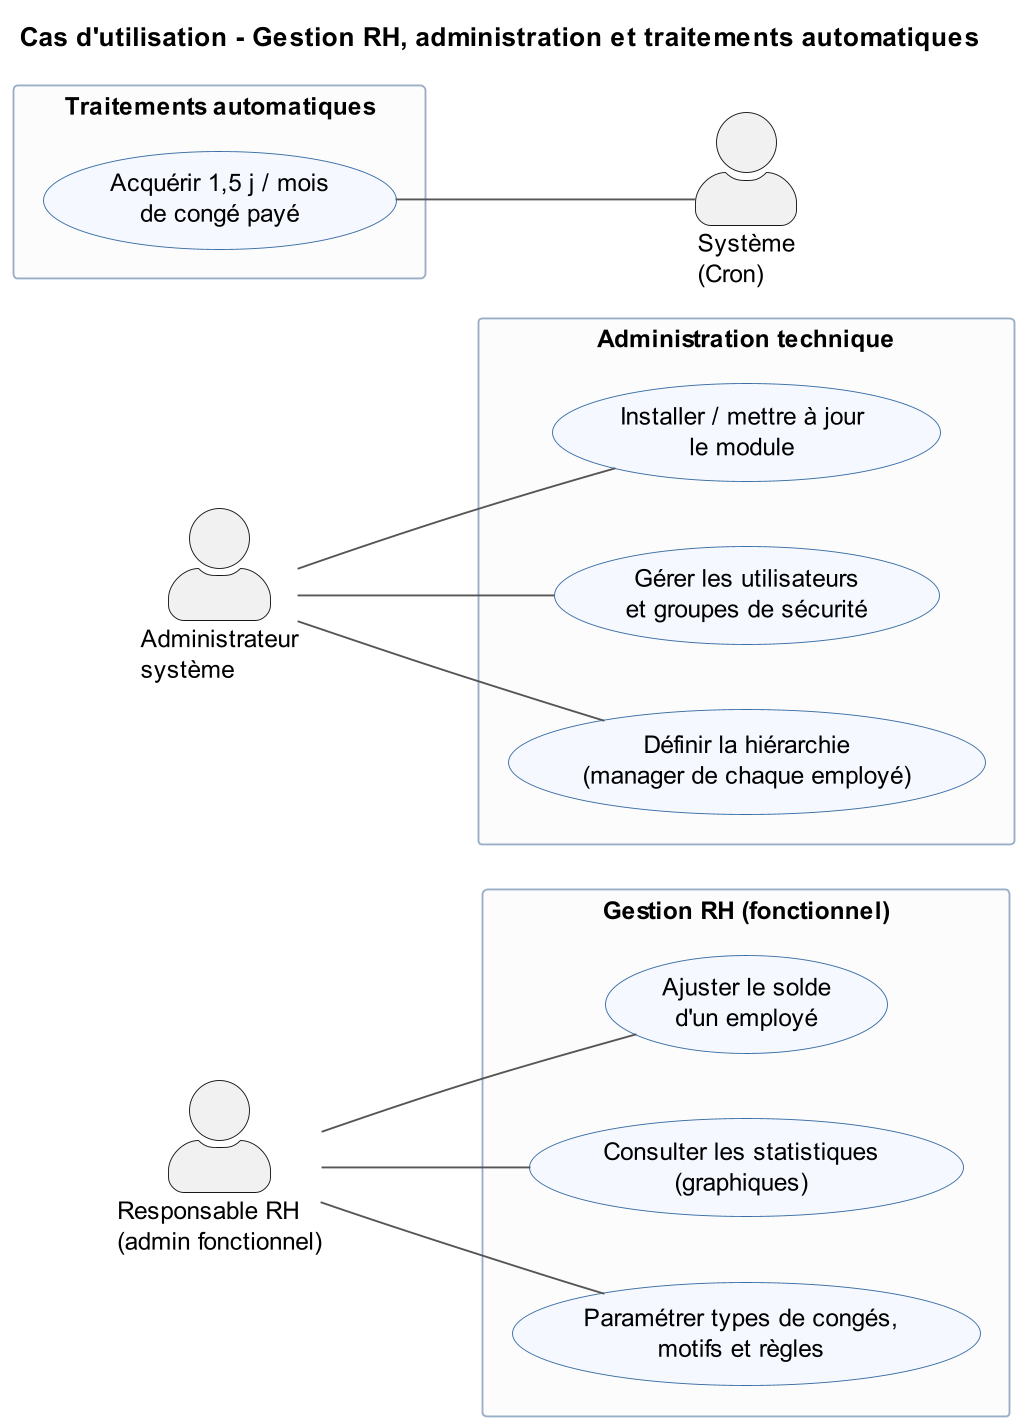
\includegraphics[width=0.62\textwidth]{img/uml/uc_3_administration.png}
\caption{Gestion RH (fonctionnelle), administration technique et traitement automatique mensuel.}
\label{fig:uc3}
\end{figure}

\subsection{Diagramme de classes}
Le cahier des charges demande de distinguer les classes Odoo réutilisées, celles qui sont étendues
par héritage (\code{_inherit}) et celles qui sont créées (\code{_name}). La figure~\ref{fig:classes}
utilise une couleur par catégorie ; le tableau~\ref{tab:classes} en donne la synthèse.

\begin{figure}[H]
\centering
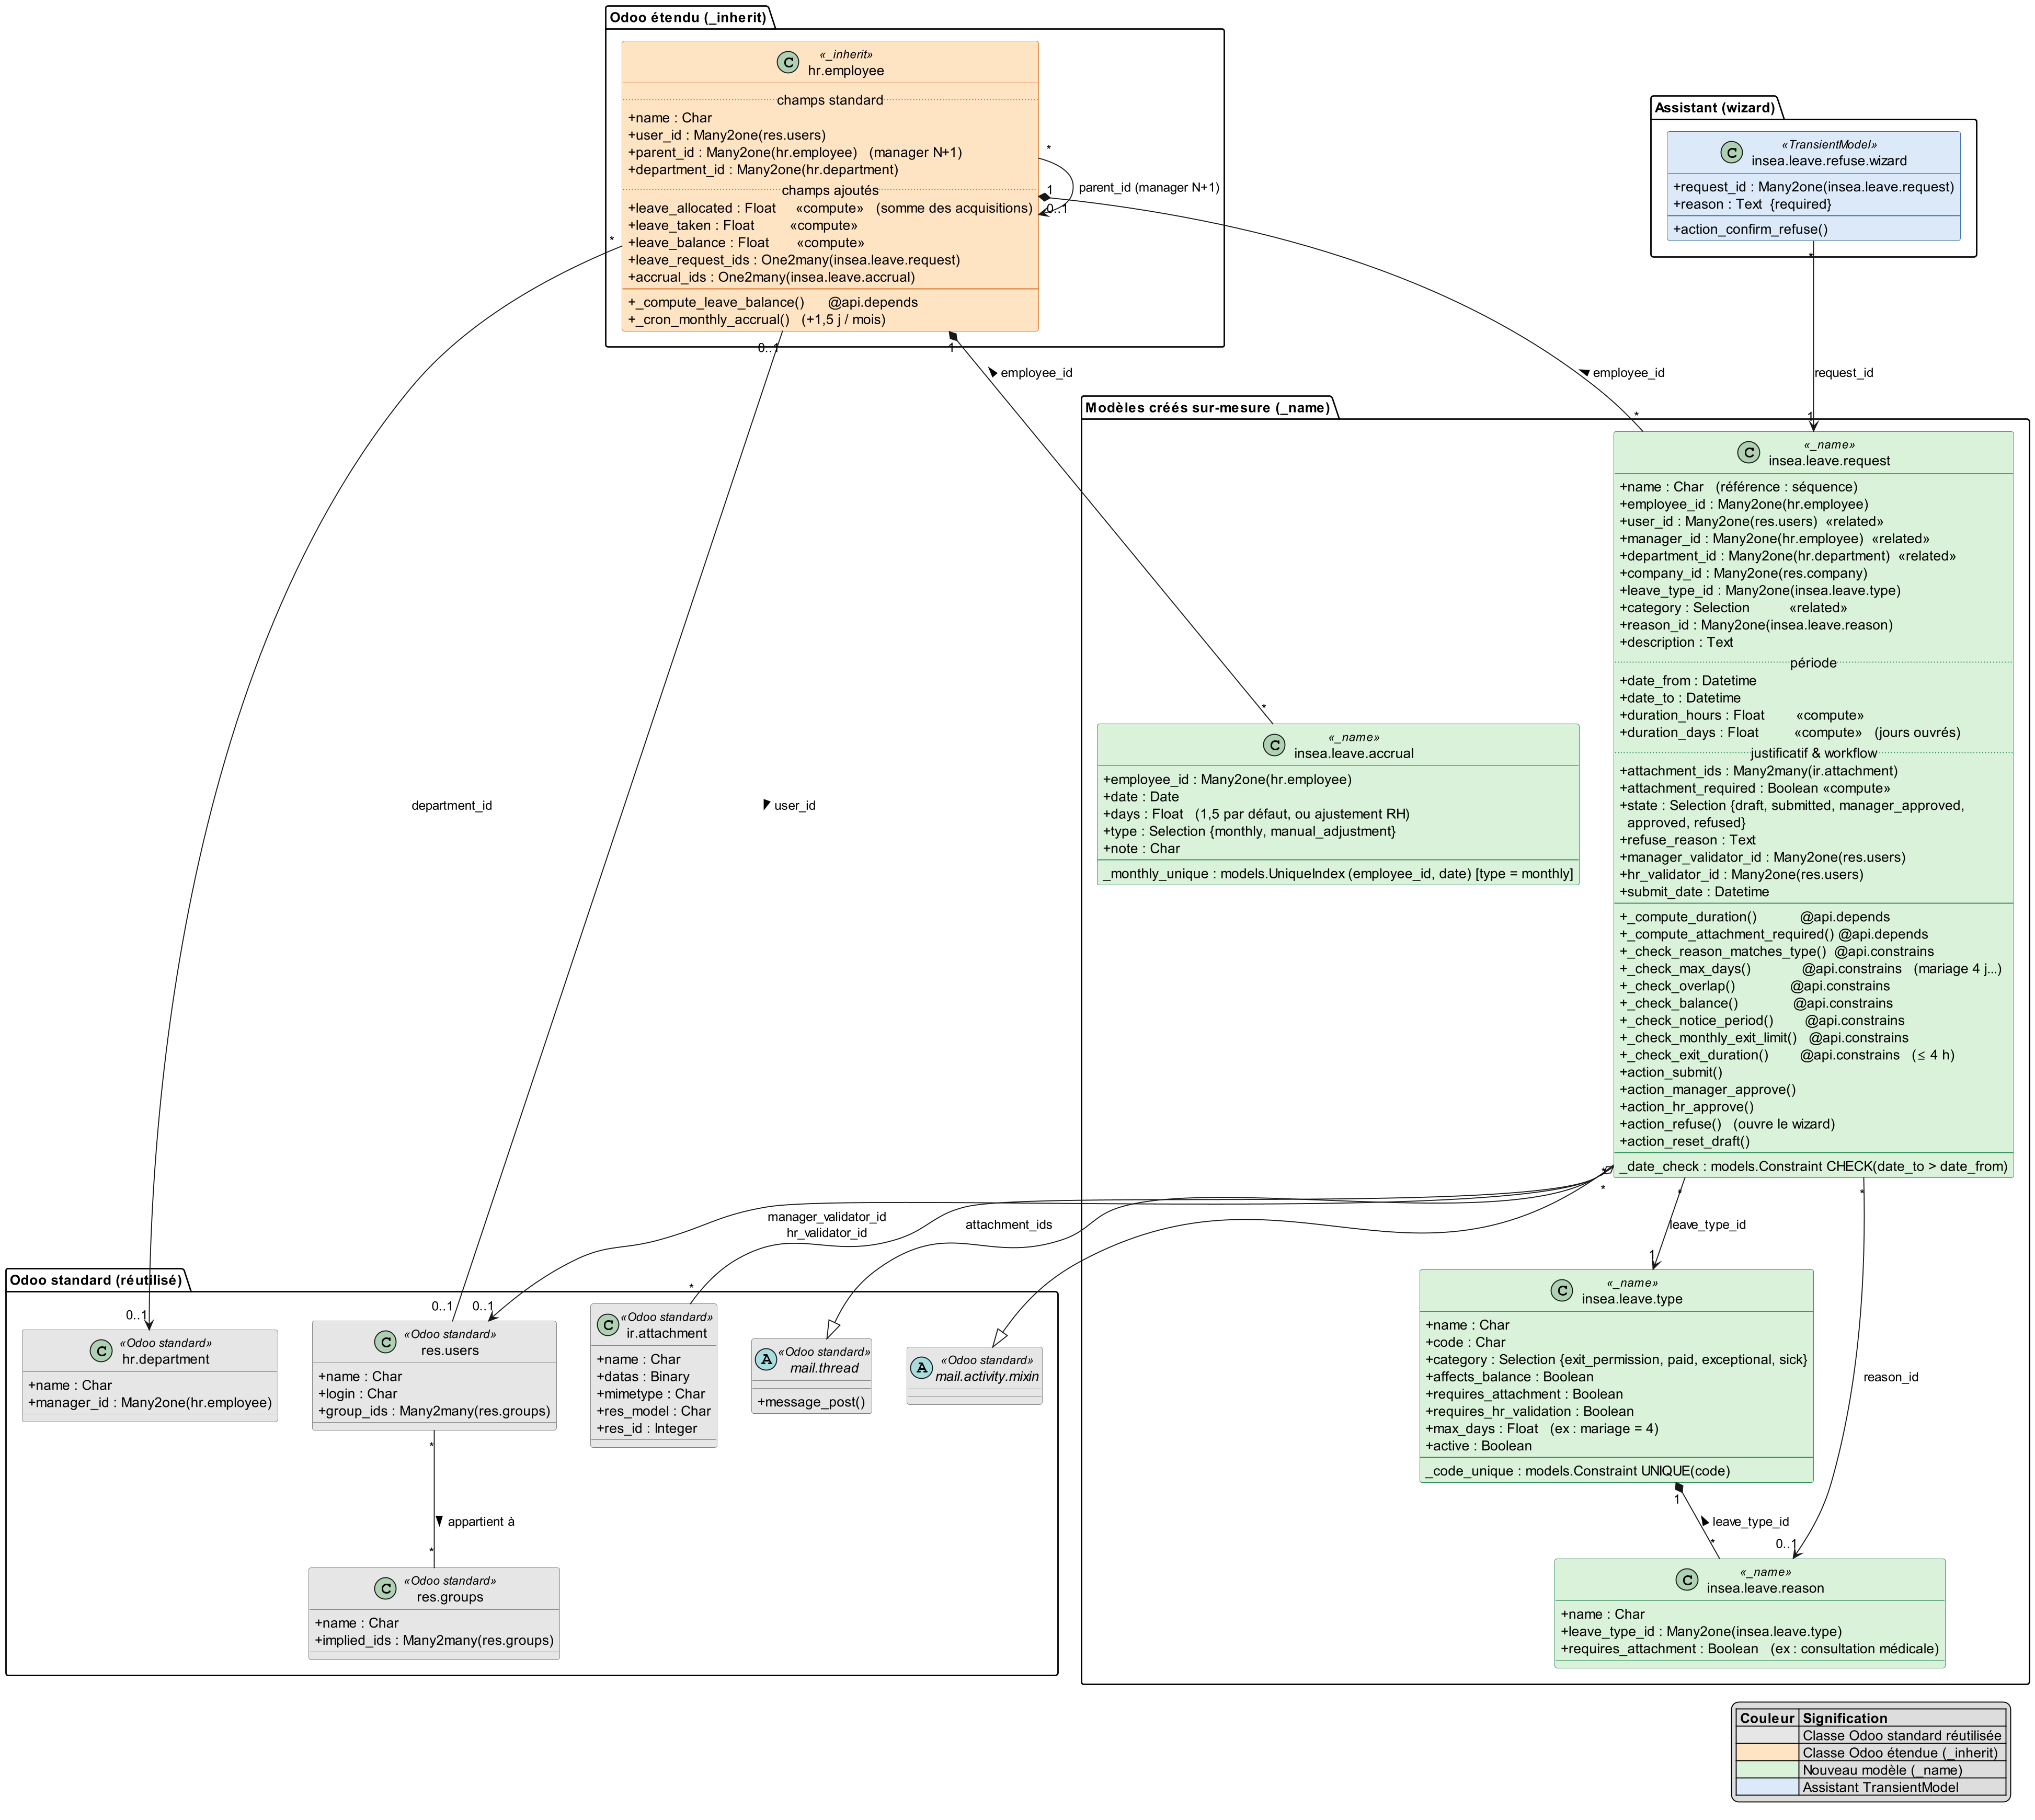
\includegraphics[width=\textwidth]{img/uml/diagramme_classes.png}
\caption{Diagramme de classes. Gris : classes Odoo réutilisées ; orange : classe étendue
(\code{_inherit}) ; vert : modèles créés (\code{_name}) ; bleu : assistant transitoire.}
\label{fig:classes}
\end{figure}

\begin{table}[H]
\centering
\caption{Classes du modèle et mode d'intégration dans Odoo.}
\label{tab:classes}
\small
\begin{tabularx}{\textwidth}{l l Y}
\toprule
Classe & Intégration & Rôle \\
\midrule
\code{res.users}, \code{res.groups} & Réutilisées & Comptes et groupes de sécurité. \\
\code{hr.department} & Réutilisée & Départements de la société. \\
\code{ir.attachment} & Réutilisée & Stockage des justificatifs. \\
\code{mail.thread}, \code{mail.activity.mixin} & Réutilisées (mixins) & Historique, messages,
activités et notifications. \\
\code{hr.employee} & Étendue (\code{_inherit}) & Ajout du solde (acquis, pris, restant), des
demandes et des acquisitions ; tâche planifiée mensuelle. \\
\code{insea.leave.request} & Créée (\code{_name}) & La demande : période, durée, justificatifs,
état, valideurs ; règles de gestion et workflow. \\
\code{insea.leave.type} & Créée (\code{_name}) & Type de demande et ses règles (déduction du solde,
justificatif, validation RH, durée maximale). \\
\code{insea.leave.reason} & Créée (\code{_name}) & Motif d'une autorisation de sortie. \\
\code{insea.leave.accrual} & Créée (\code{_name}) & Ligne d'acquisition (mensuelle ou ajustement
RH). \\
\code{insea.leave.refuse.wizard} & Créée (\code{TransientModel}) & Assistant imposant le motif de
refus. \\
\bottomrule
\end{tabularx}
\end{table}

\subsection{Diagramme d'états-transitions}
Le champ \code{state} de \code{insea.leave.request} porte le cycle de vie d'une demande
(figure~\ref{fig:etats}). Les gardes sur les transitions correspondent aux contrôles du code.

\begin{figure}[H]
\centering
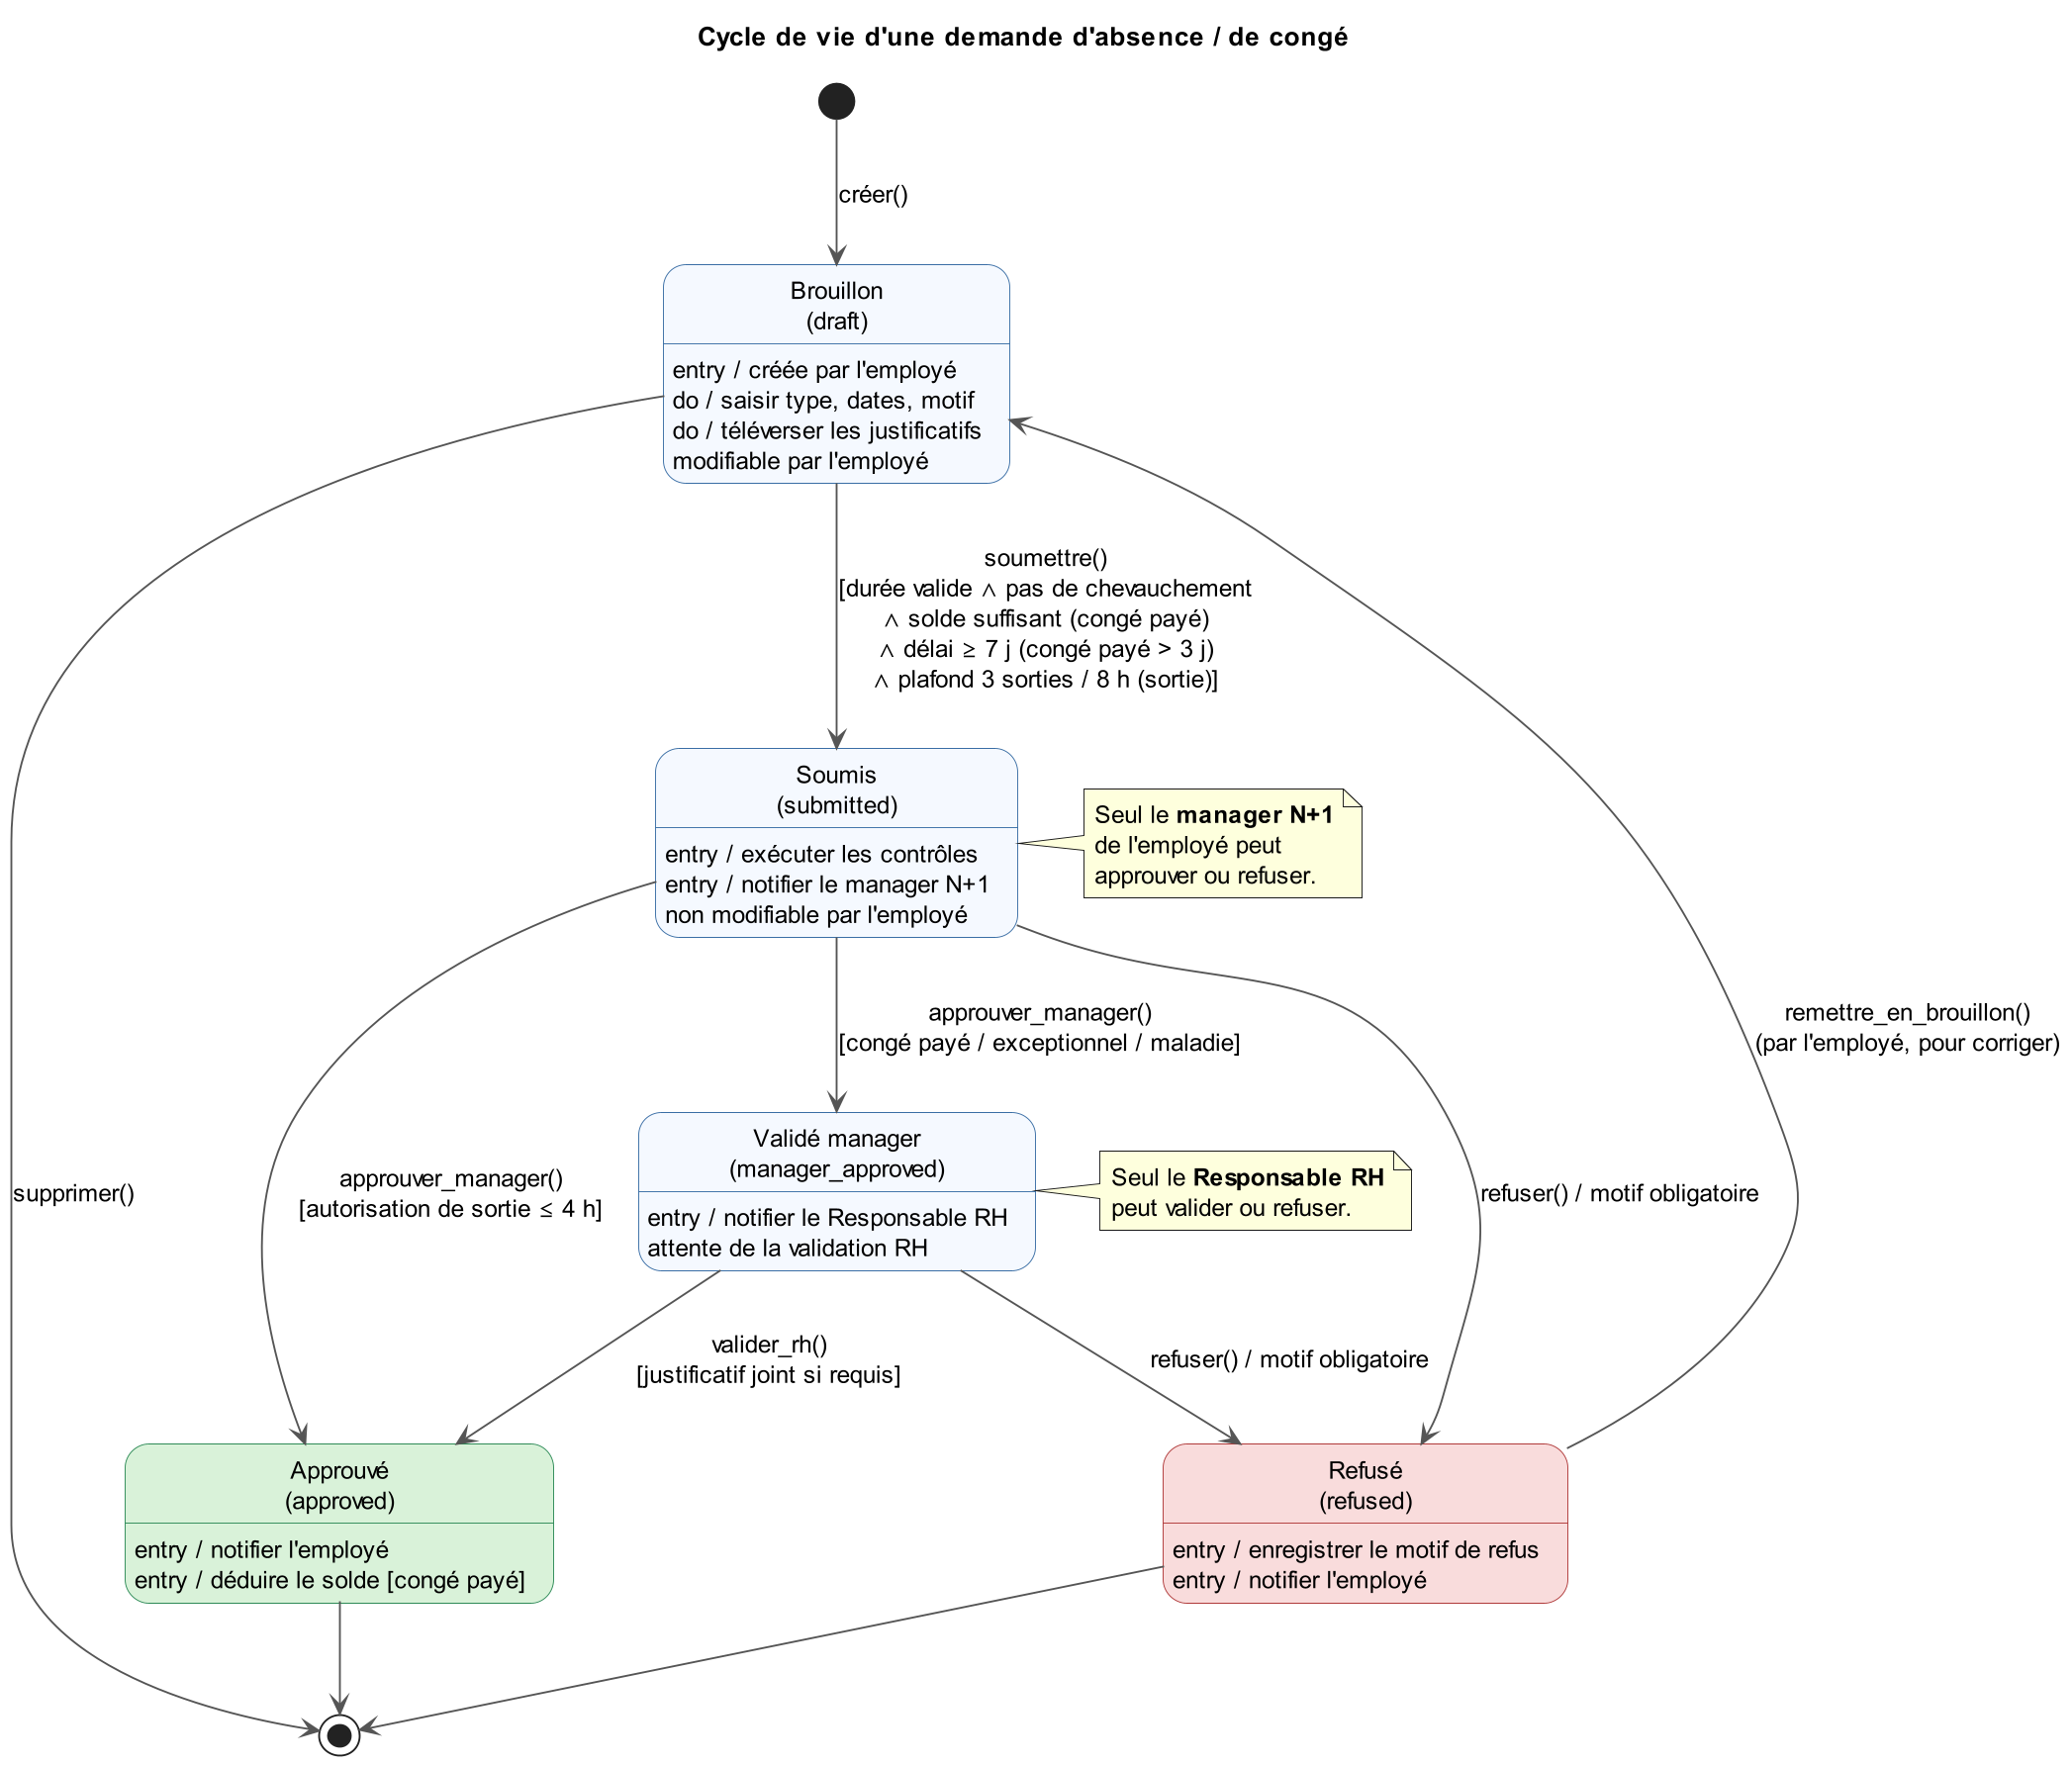
\includegraphics[width=0.92\textwidth]{img/uml/diagramme_etats_transitions.png}
\caption{Cycle de vie d'une demande. Une autorisation de sortie passe de \emph{Soumis} à
\emph{Approuvé} dès l'approbation du manager ; un congé passe par \emph{Validé manager} avant la
validation RH.}
\label{fig:etats}
\end{figure}

\subsection{Diagramme de séquence}
La figure~\ref{fig:sequence} détaille les échanges lors de la soumission puis de la validation d'un
congé payé. Les messages portent les noms réels des méthodes du module.

\begin{figure}[H]
\centering
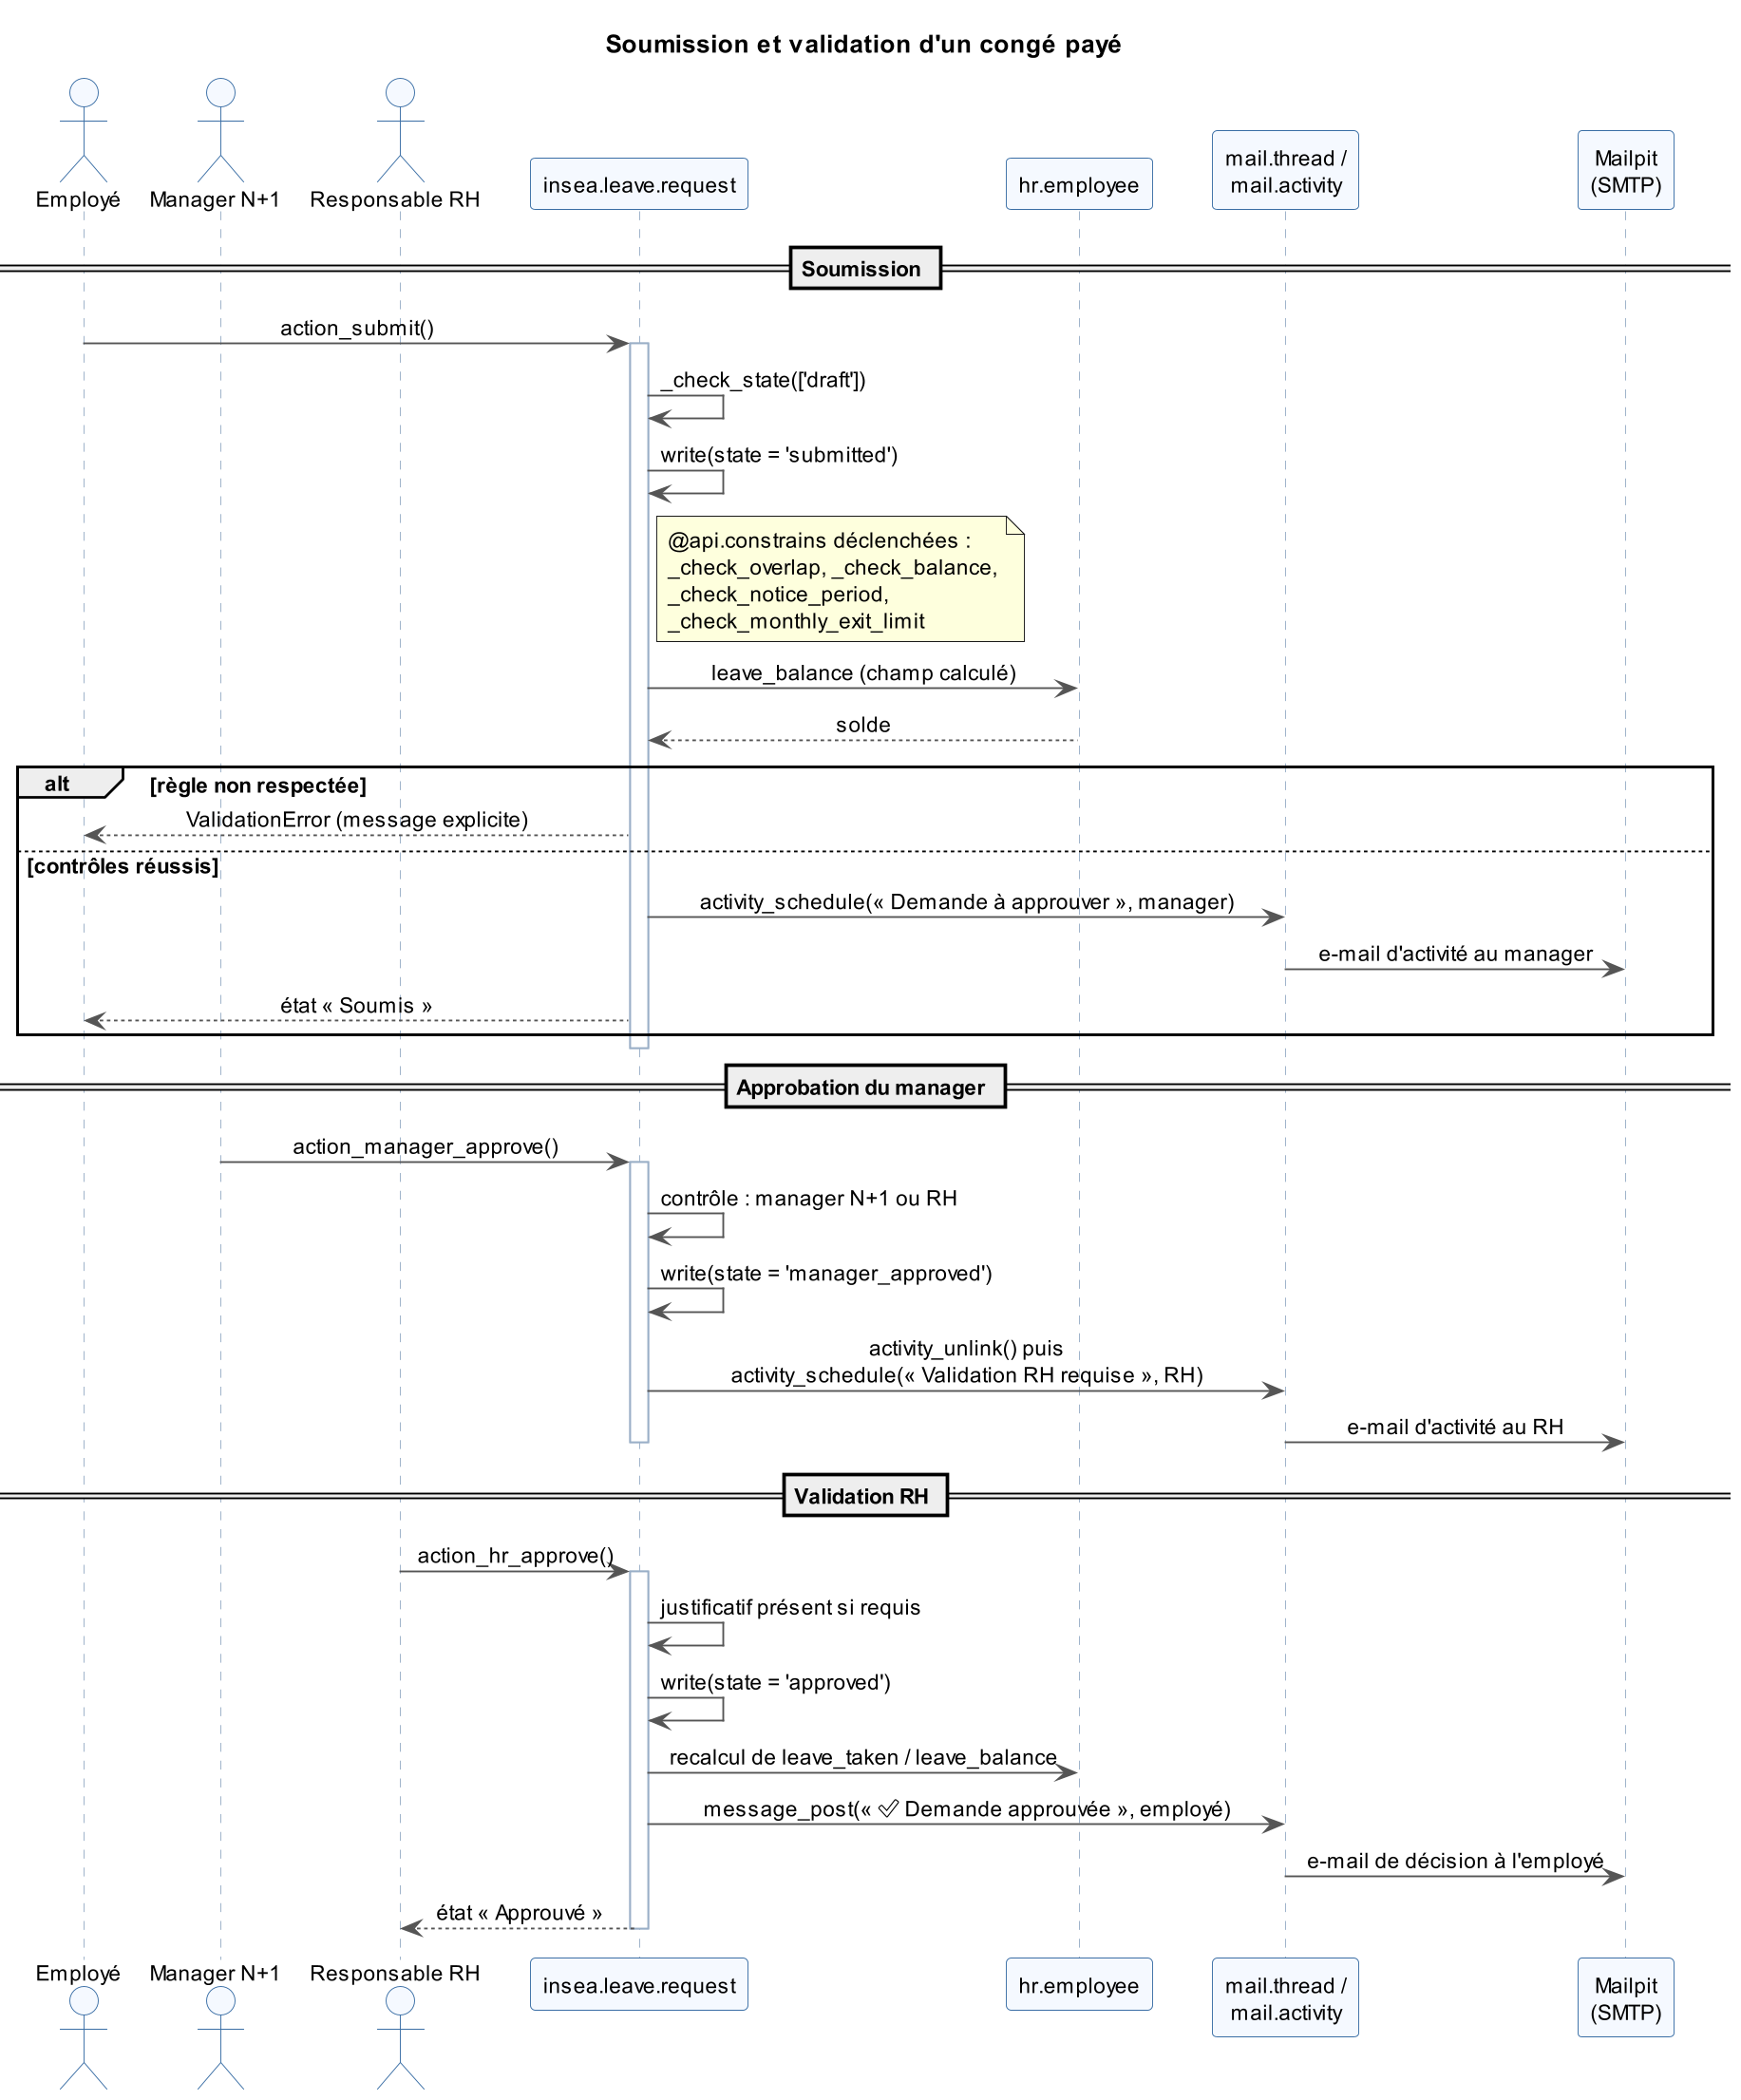
\includegraphics[width=0.86\textwidth]{img/uml/diagramme_sequence.png}
\caption{Séquence de soumission et de validation d'un congé payé. Les contraintes
\code{@api.constrains} se déclenchent à l'écriture de l'état \emph{submitted} ; une violation lève
une \code{ValidationError} et annule l'opération.}
\label{fig:sequence}
\end{figure}

% =====================================================================
\section{Architecture technique}\label{sec:archi}
% =====================================================================

\subsection{Pile logicielle}
L'application est déployée avec Docker Compose. La pile comprend trois conteneurs reliés par un
réseau privé (figure~\ref{fig:deploiement} et tableau~\ref{tab:conteneurs}).

\begin{figure}[H]
\centering
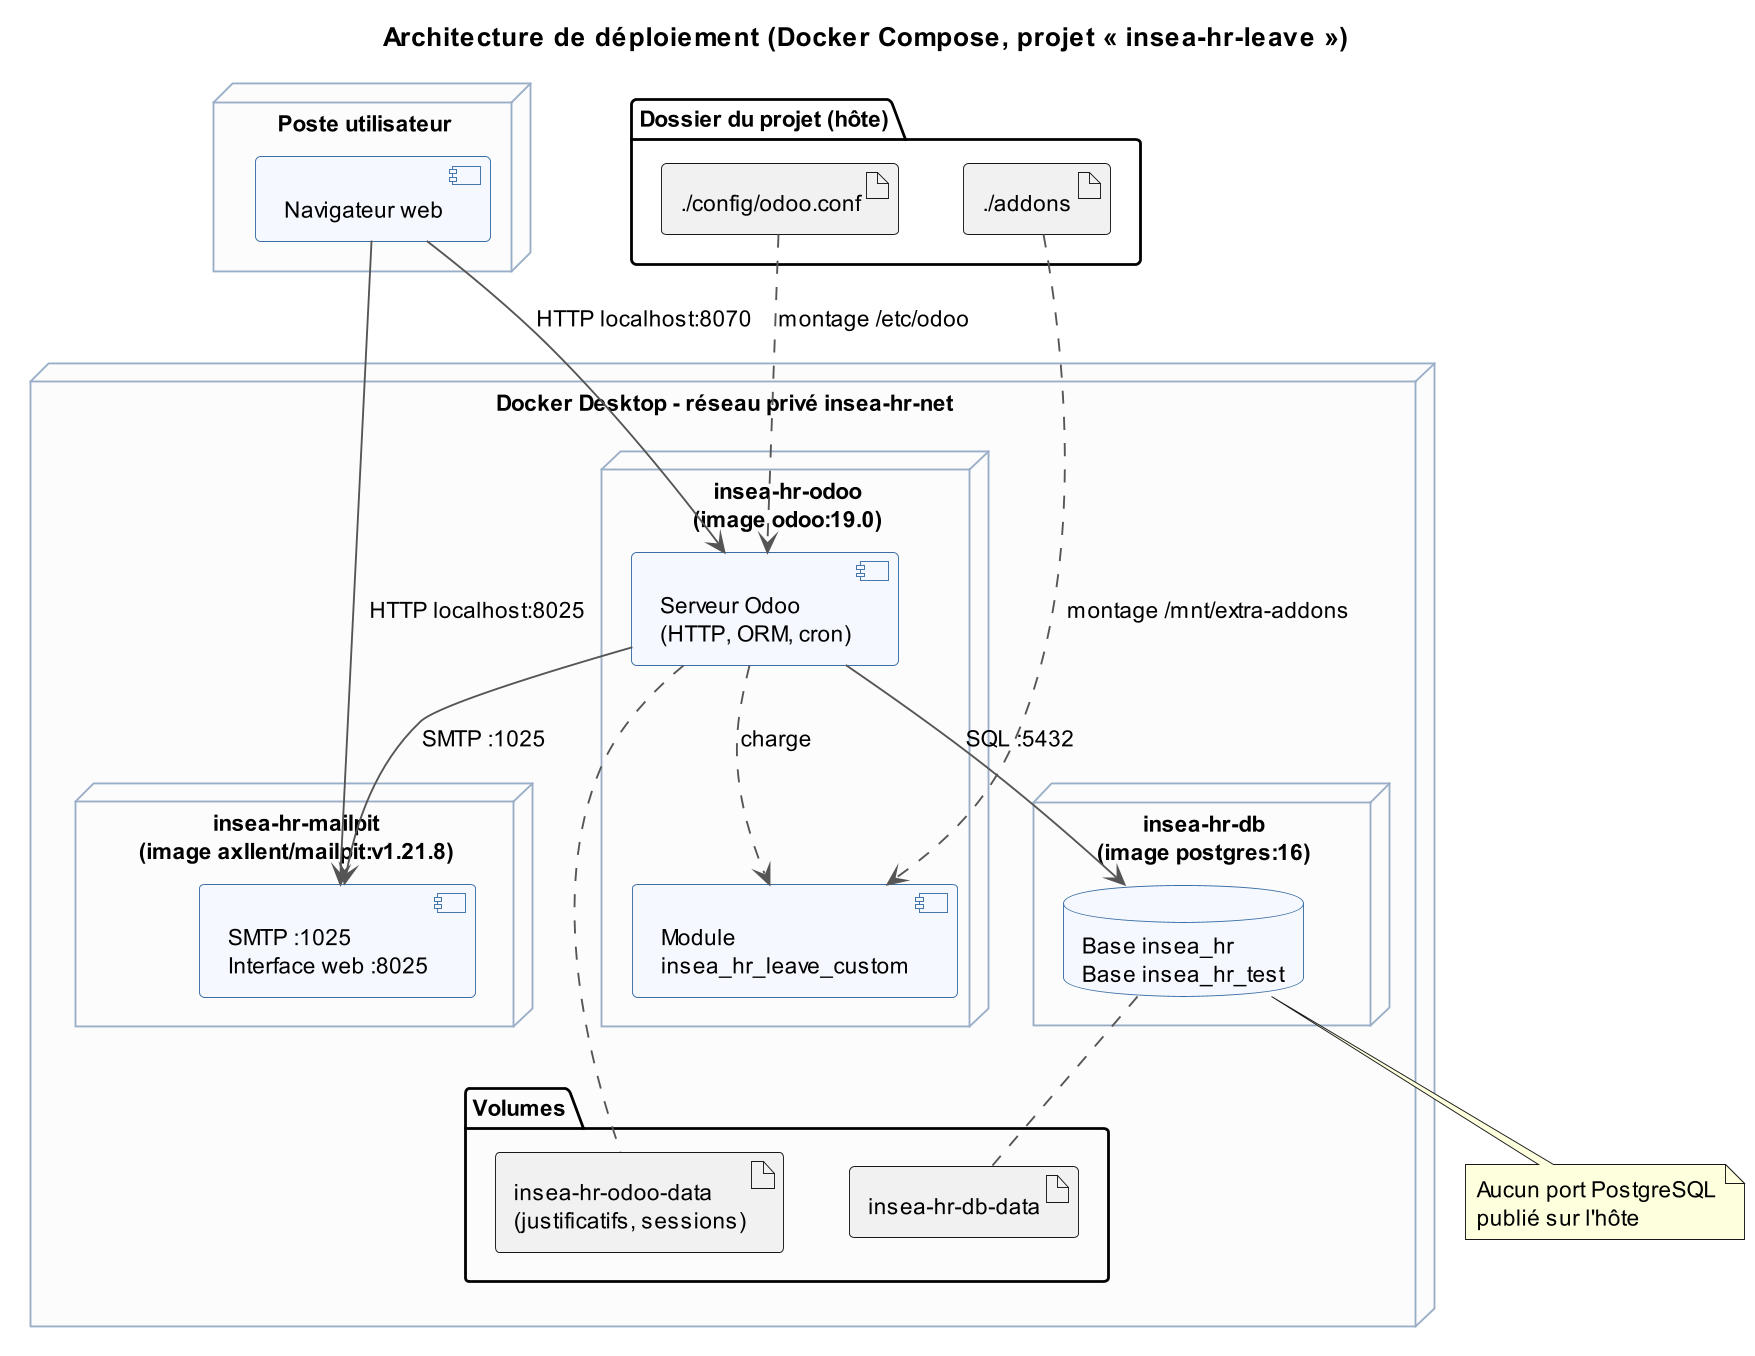
\includegraphics[width=0.85\textwidth]{img/uml/diagramme_deploiement.png}
\caption{Diagramme de déploiement de la pile Docker Compose.}
\label{fig:deploiement}
\end{figure}

\begin{table}[H]
\centering
\caption{Composants de la pile Docker.}
\label{tab:conteneurs}
\small
\begin{tabularx}{\textwidth}{l l l Y}
\toprule
Conteneur & Image & Port hôte & Rôle \\
\midrule
\code{insea-hr-odoo} & \code{odoo:19.0} & 8070 & Serveur Odoo (interface web, ORM, tâches planifiées) ;
charge le module depuis \code{./addons}. \\
\code{insea-hr-db} & \code{postgres:16} & aucun & Bases \code{insea_hr} (démonstration) et
\code{insea_hr_test} (tests). \\
\code{insea-hr-mailpit} & \code{axllent/mailpit:v1.21.8} & 8025 & Serveur SMTP factice : capture
les e-mails d'Odoo et les affiche dans une boîte web. \\
\bottomrule
\end{tabularx}
\end{table}

La version exacte du serveur est \code{19.0-20261015}. Les volumes nommés
\code{insea-hr-db-data} et \code{insea-hr-odoo-data} conservent respectivement la base PostgreSQL
et le \emph{filestore} (justificatifs téléversés).

\subsection{Choix d'architecture}
\begin{itemize}
  \item \textbf{Isolation} : le projet Compose (\code{insea-hr-leave}), les conteneurs, les volumes
        et le réseau sont préfixés \code{insea-hr}, et le port d'Odoo est 8070 au lieu de 8069. Le
        projet peut ainsi tourner en même temps qu'un autre projet Odoo.
  \item \textbf{Base de données non exposée} : aucun port PostgreSQL n'est publié sur l'hôte ; seul
        Odoo y accède, par le réseau Docker.
  \item \textbf{E-mails capturés} : \code{config/odoo.conf} déclare \code{smtp_server = mailpit} et
        \code{smtp_port = 1025}. Les notifications peuvent ainsi être démontrées sans qu'aucun
        message ne parte sur Internet.
  \item \textbf{Secrets hors du code} : les mots de passe sont dans \code{.env} et
        \code{config/odoo.conf}, exclus du suivi de version ; des modèles \code{.example} sont
        fournis.
\end{itemize}

% =====================================================================
\section{Implémentation dans Odoo}\label{sec:impl}
% =====================================================================

\subsection{Choix de conception : un modèle dédié}
Odoo propose une application de congés (\code{hr_holidays}, modèle \code{hr.leave}). Nous avons
choisi de ne pas l'étendre et de créer un modèle dédié, \code{insea.leave.request}, pour trois
raisons :
\begin{enumerate}
  \item le cahier des charges impose ses propres états (dont \emph{Validé manager}) et ses propres
        règles, qu'il est plus sûr de maîtriser entièrement que de greffer sur un workflow existant ;
  \item la distinction demandée entre classes réutilisées, étendues et créées est plus nette ;
  \item le module ne dépend que de \code{hr} et de \code{mail}, ce qui limite les interactions avec
        d'autres applications.
\end{enumerate}
Le modèle standard \code{hr.employee} est en revanche étendu, car le solde de congés est une
propriété naturelle de l'employé.

\subsection{Structure du module}

\begin{figure}[H]
\centering
\begin{minipage}[c]{0.36\textwidth}
  \centering
  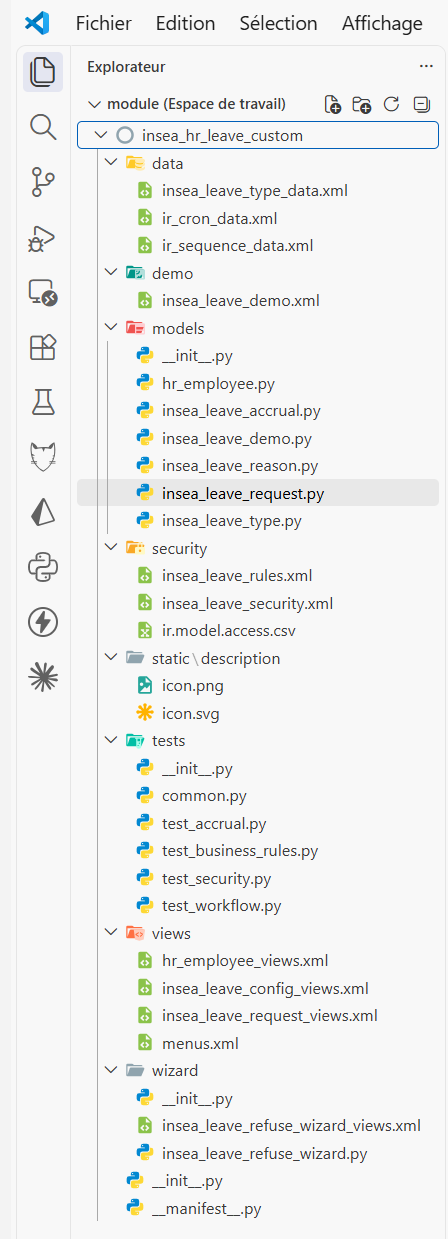
\includegraphics[width=\linewidth]{img/vscode_arborescence.png}
\end{minipage}\hfill
\begin{minipage}[c]{0.60\textwidth}
  \small
  \begin{tabularx}{\linewidth}{>{\ttfamily}l Y}
  \toprule
  \normalfont Dossier & Contenu \\
  \midrule
  data/ & Types et motifs, séquence \code{DA/}, tâche planifiée mensuelle. \\
  demo/ & Appel du chargeur de la société Lambda. \\
  models/ & Les cinq modèles métier et l'extension de \code{hr.employee}. \\
  security/ & Groupes, droits d'accès, règles d'enregistrement. \\
  static/ & Icône de l'application (SVG et PNG). \\
  tests/ & 49 tests automatisés et leurs données communes. \\
  views/ & Vues, actions, menus et héritage de la fiche employé. \\
  wizard/ & Assistant de refus (\code{TransientModel}). \\
  \_\_manifest\_\_.py & Métadonnées ; dépendances \code{hr} et \code{mail}. \\
  \bottomrule
  \end{tabularx}
\end{minipage}
\caption{Arborescence du module \texttt{insea\_hr\_leave\_custom} dans l'explorateur de Visual Studio
Code, et rôle de chaque dossier.}
\label{fig:arbo}
\end{figure}

Le module totalise environ 2\,400 lignes : 1\,012 lignes de Python pour les modèles, 602 lignes de
XML pour les vues et 554 lignes de tests.

\subsection{Modèles et champs}
\subsubsection{La demande (\code{insea.leave.request})}
Le modèle hérite de \code{mail.thread} et \code{mail.activity.mixin} ; il compte 28 champs. Les
principaux sont :
\begin{itemize}
  \item \textbf{identification} : \code{name}, la référence issue de la séquence
        \texttt{DA/\%(year)s/} sur 4 chiffres, et \code{employee_id}. Les champs liés et stockés
        \code{user_id}, \code{manager_id} (lié à \code{employee_id.parent_id}) et
        \code{department_id} servent aux règles d'accès et aux filtres ;
  \item \textbf{période} : \code{date_from}, \code{date_to}, \code{duration_hours},
        \code{duration_days} ;
  \item \textbf{justificatifs et workflow} : \code{attachment_ids}, \code{attachment_required},
        \code{state}, \code{submit_date}, \code{manager_validator_id}, \code{hr_validator_id},
        \code{refuse_reason}.
\end{itemize}

\subsubsection{Champs calculés (\code{@api.depends})}
\begin{table}[H]
\centering
\caption{Champs calculés du module.}
\small
\begin{tabularx}{\textwidth}{l l Y}
\toprule
Méthode & Dépendances & Calcul \\
\midrule
\code{_compute_duration} & dates, catégorie & Sortie : durée en heures. Congé : nombre de jours
ouvrés, du lundi au vendredi, bornes incluses. Une seule unité par catégorie, pour des totaux
cohérents. \\
\code{_compute_attachment_required} & type, motif & Vrai si le type ou le motif exige un
justificatif. \\
\code{_compute_user_rights} & état, utilisateur courant & Droits d'affichage des boutons
(\code{can_manager_approve}, \code{can_hr_approve}, \code{can_refuse}, \code{is_owner}). \\
\code{_compute_display_name} & référence, employé, type & Libellé lisible, par exemple
\emph{DA/2026/0085 -- Omar Fassi (Congé payé annuel)}. \\
\code{_compute_leave_balance} & acquisitions, demandes approuvées & Sur \code{hr.employee} :
acquis $-$ pris = solde. \\
\bottomrule
\end{tabularx}
\end{table}

\subsection{Contraintes et règles de gestion}
Les règles du tableau~\ref{tab:regles} sont implémentées par des contraintes Python
(\code{@api.constrains}) et par des contraintes SQL. Les contraintes Python déclarées sur le champ
\code{state} ne s'appliquent qu'au passage à l'état concerné : elles réalisent donc les contrôles
\og à la soumission \fg{}.

\begin{table}[H]
\centering
\caption{Contraintes implémentées dans le modèle de demande.}
\label{tab:contraintes}
\small
\begin{tabularx}{\textwidth}{l >{\raggedright\arraybackslash}p{3.7cm} Y}
\toprule
Méthode & Déclencheur & Règle vérifiée \\
\midrule
\code{_check_exit_duration} & dates, type & Sortie le même jour et d'au plus 4~h. \\
\code{_check_max_days} & dates, type & Durée inférieure ou égale au maximum du type (mariage 4~j,
naissance 3~j, décès 3~j). \\
\code{_check_overlap} & dates, employé, état & Aucun recouvrement avec une demande soumise, en
validation ou approuvée du même employé. \\
\code{_check_reason_matches_type} & motif, type & Le motif appartient au type choisi. \\
\code{_check_monthly_exit_limit} & état = soumis & Au plus 3 sorties ou 8~h dans le mois de début
de la sortie. \\
\code{_check_balance} & état = soumis ou validé manager & Solde disponible $\geq$ durée demandée. \\
\code{_check_notice_period} & état = soumis & Congé payé de plus de 3~jours : début au moins
7~jours après la date du jour. \\
\bottomrule
\end{tabularx}
\end{table}

Le contrôle du solde tient compte des autres congés payés déjà en attente : deux demandes en cours
ne peuvent pas consommer les mêmes jours.


\begin{figure}[H]
\centering
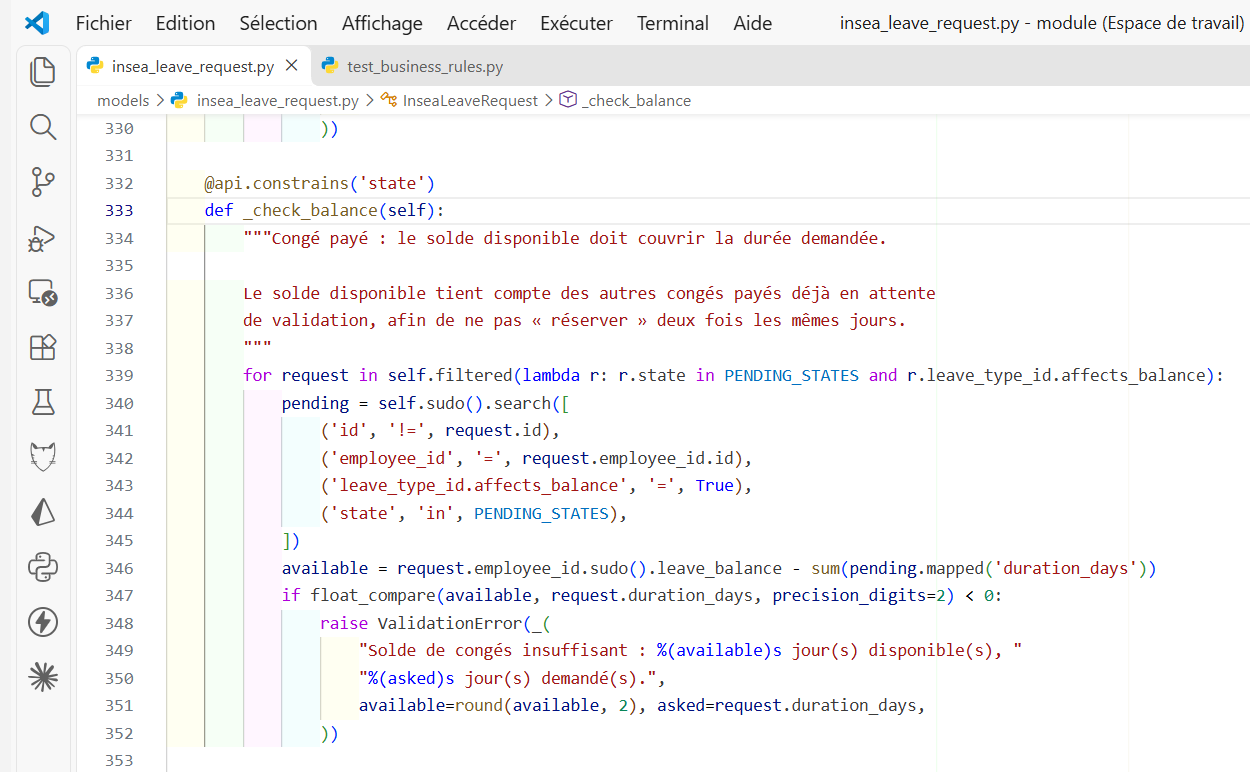
\includegraphics[width=0.94\textwidth]{img/vscode_check_balance.png}
\caption{Contrainte \code{_check_balance} dans \code{models/insea_leave_request.py} (Visual Studio
Code, lignes 332 à 352). Les congés payés en attente sont déduits du solde avant la comparaison.}
\label{fig:code_balance}
\end{figure}

Les contraintes SQL utilisent la syntaxe d'Odoo~19 (\code{models.Constraint} et
\code{models.UniqueIndex}, qui remplacent \code{_sql_constraints}) :

\begin{table}[H]
\centering
\caption{Contraintes SQL.}
\small
\begin{tabularx}{\textwidth}{l Y >{\raggedright\arraybackslash}p{5.2cm}}
\toprule
Modèle & Contrainte & Effet \\
\midrule
\code{insea.leave.request} & \code{CHECK (date_to > date_from)} & La fin suit le début. \\
\code{insea.leave.type} & \code{UNIQUE (code)} & Codes de type uniques. \\
\code{insea.leave.type} & \code{CHECK (max_days >= 0)} & Durée maximale positive. \\
\code{insea.leave.accrual} & index unique partiel \code{(employee_id, date)} si \code{type = 'monthly'}
& Une seule acquisition mensuelle par employé et par mois. \\
\bottomrule
\end{tabularx}
\end{table}

\subsection{Workflow}
Le workflow est porté par des méthodes appelées depuis les boutons du formulaire. Chacune vérifie
l'état de départ (\code{_check_state}) et le rôle de l'utilisateur avant d'écrire le nouvel état.

\begin{table}[H]
\centering
\caption{Méthodes du workflow.}
\small
\begin{tabularx}{\textwidth}{l l Y}
\toprule
Méthode & Transition & Contrôles et effets \\
\midrule
\code{action_submit} & Brouillon $\rightarrow$ Soumis & Auteur ou RH ; contraintes de soumission ;
activité \og Demande à approuver \fg{} pour le manager. \\
\code{action_manager_approve} & Soumis $\rightarrow$ Approuvé ou Validé manager & Manager N+1 ou RH ;
finale si le type n'exige pas de validation RH (sortie) ; sinon activité \og Validation RH requise
\fg{}. \\
\code{action_hr_approve} & Validé manager $\rightarrow$ Approuvé & RH uniquement ; justificatif
présent si requis ; e-mail à l'employé (avec le nouveau solde pour un congé payé). \\
\code{action_refuse} & ouvre l'assistant & L'assistant exige un motif non vide ; manager ou RH au
stade \emph{Soumis}, RH seul au stade \emph{Validé manager}. \\
\code{action_reset_draft} & Refusé $\rightarrow$ Brouillon & Auteur ou RH ; efface le motif et les
valideurs pour une nouvelle soumission. \\
\bottomrule
\end{tabularx}
\end{table}

Une demande ne peut être supprimée qu'à l'état \emph{Brouillon} (surcharge de \code{unlink}).

\subsection{Sécurité}\label{sec:securite}
\subsubsection{Groupes}
Les trois groupes du module sont rattachés à un \code{res.groups.privilege} (mécanisme introduit par
Odoo~19) et s'emboîtent par \code{implied_ids} :
\begin{center}
\small
\begin{tabular}{l l}
\toprule
Groupe & Implique \\
\midrule
Employé (\code{group_leave_employee}) & \code{base.group_user} \\
Manager N+1 (\code{group_leave_manager}) & Employé \\
Responsable RH (\code{group_leave_hr}) & Manager, \code{hr.group_hr_user} \\
\bottomrule
\end{tabular}
\end{center}
Le groupe RH implique le groupe standard \og Employés : Officier \fg{} afin que le RH puisse ouvrir
les fiches employés et gérer les soldes. L'Administrateur système correspond au groupe standard
\code{base.group_system}.

\subsubsection{Droits d'accès (\code{ir.model.access.csv})}
\begin{table}[H]
\centering
\caption{Droits d'accès par modèle (L = lecture, É = écriture, C = création, S = suppression).}
\small
\begin{tabular}{l c c c}
\toprule
Modèle & Employé & Manager & Responsable RH \\
\midrule
\code{insea.leave.request} & L É C S & L É C S & L É C S \\
\code{insea.leave.type}, \code{insea.leave.reason} & L & L & L É C S \\
\code{insea.leave.accrual} & L & L & L É C S \\
\code{insea.leave.refuse.wizard} & -- & L É C & L É C \\
\bottomrule
\end{tabular}
\end{table}

\subsubsection{Règles d'enregistrement}
Les règles de groupes différents s'additionnent (OU logique). Le périmètre de chaque rôle est donc
l'union des règles de ses groupes.
\begin{table}[H]
\centering
\caption{Règles d'enregistrement sur les demandes.}
\small
\begin{tabularx}{\textwidth}{l l Y}
\toprule
Règle & Groupe & Domaine \\
\midrule
Ses propres demandes & Employé & \code{[('employee_id.user_id', '=', user.id)]} \\
Demandes de l'équipe & Manager & \code{[('employee_id.parent_id.user_id', '=', user.id)]}
(lecture et écriture, sans création ni suppression) \\
Toutes les demandes & Responsable RH & \code{[(1, '=', 1)]} \\
Multi-société & globale & \code{[('company_id', 'in', company_ids)]} \\
\bottomrule
\end{tabularx}
\end{table}
Des règles analogues limitent la lecture des acquisitions : l'employé voit les siennes, le RH
toutes.

\subsection{Interfaces XML}
Les vues sont écrites avec la syntaxe d'Odoo~19 : balise \code{<list>} au lieu de \code{<tree>},
attributs \code{invisible}, \code{readonly} et \code{required} portant une expression (les attributs
\code{attrs} et \code{states} n'existent plus).
\begin{itemize}
  \item \textbf{Formulaire} : barre de statut, boutons conditionnés par les champs de droits,
        bandeaux \og Approuvé \fg{} / \og Refusé \fg{}, rappel des règles selon le type, alerte si
        le justificatif manque, onglets Justificatifs, Commentaire et Suivi de validation, chatter.
  \item \textbf{Liste}, \textbf{kanban} (colonnes par état), \textbf{calendrier} (départs, couleur
        par employé), \textbf{tableau croisé} et \textbf{graphique} (jours par type et par mois).
  \item \textbf{Recherche} : filtres \emph{Mes demandes}, \emph{Mon équipe}, \emph{À approuver},
        \emph{À valider (RH)}, états, sorties ou congés, date ; regroupements par employé,
        département, type, état et mois.
  \item \textbf{Fiche employé} : onglet \og Congés \fg{} ajouté par héritage de vue
        (\code{hr.view_employee_form}), visible par le RH.
  \item \textbf{Menus} : chaque entrée porte son groupe ; un employé ne voit que \emph{Mes
        demandes}.
\end{itemize}

\subsection{Notifications et tâche planifiée}
Les notifications s'appuient sur les mixins de messagerie d'Odoo :
\begin{itemize}
  \item à la soumission, une activité \og Demande à approuver \fg{} est créée pour le manager (ou
        pour le RH si l'employé n'a pas de manager) ;
  \item après l'approbation du manager, l'activité passe au RH ;
  \item la décision finale (approbation ou refus avec motif) est publiée dans le chatter et adressée
        à l'employé (\code{message_post} avec \code{partner_ids}), avec un objet explicite.
\end{itemize}
La tâche planifiée \og acquisition mensuelle \fg{} appelle \code{hr.employee._cron_monthly_accrual()}
le 1\textsuperscript{er} de chaque mois à 2~h. Elle crédite 1,5~jour à chaque employé actif. Une
ligne déjà créée pour le mois n'est jamais dupliquée : la méthode le vérifie, et l'index unique
partiel l'interdit en base.

\subsection{Données de référence}
Le module installe les types \code{SORTIE}, \code{CP}, \code{EXC_MAR} (4~j), \code{EXC_NAI} (3~j),
\code{EXC_DEC} (3~j) et \code{MAL}, ainsi que trois motifs de sortie : consultation médicale
(justificatif obligatoire), démarche administrative et urgence personnelle. Ces données sont
déclarées \code{noupdate} : les modifications faites par le RH sont conservées lors des mises à
jour.

% =====================================================================
\section{Présentation de l'application}\label{sec:ihm}
% =====================================================================
Les captures suivantes proviennent de la base de démonstration (section~\ref{sec:demo}). Elles ont
été réalisées le 16 novembre 2026 ; les dates des demandes sont calculées à partir de ce jour.

\subsection{Parcours de l'employé}
\fig{img/03_employe_mes_demandes.png}{Vue \emph{Mes demandes} de Karim Idrissi (employé). Les
heures ne s'affichent que pour les sorties et les jours que pour les congés.}

\fig{img/05_erreur_sortie_5h.png}{\label{fig:err5h}Saisie d'une sortie de 5~heures : la contrainte
\code{_check_exit_duration} bloque l'enregistrement. Le bandeau bleu rappelle les règles des
sorties.}

\subsection{Parcours du manager}
\fig{img/06_manager_a_valider.png}{Menu \emph{Demandes à valider} de Youssef Alaoui : uniquement les
demandes de son équipe, sans ses propres demandes.}

\fig{img/07_manager_formulaire_soumis.png}{Demande soumise vue par le manager : boutons
\emph{Approuver} et \emph{Refuser}, solde de l'employé, activité \og Demande à approuver \fg{} dans le
chatter.}

\fig[0.82\textwidth]{img/08_assistant_refus.png}{Assistant de refus : le motif est obligatoire.}

\subsection{Parcours du Responsable RH}
\fig{img/15_rh_justificatif_manquant.png}{Congé de naissance validé par le manager mais sans
justificatif : l'alerte jaune signale le blocage de la validation RH.}

\fig{img/17_demande_approuvee.png}{Congé payé approuvé : bandeau vert et historique complet de la
création à la validation RH, avec le nombre de jours déduits et le nouveau solde.}

\fig{img/21_fiche_employe_conges.png}{Onglet \emph{Congés} de la fiche employé : acquis, pris,
solde et historique des acquisitions mensuelles.}

\subsection{Visibilité et pilotage}
\fig{img/12_calendrier.png}{Calendrier des absences (demandes soumises, en validation et
approuvées), avec filtres par employé et par type.}

\fig{img/13_graphique.png}{Analyse des absences approuvées : jours ouvrés par mois et par type. Les
sorties, comptées en heures, n'apparaissent pas dans cette mesure en jours.}

\fig{img/11_rh_kanban.png}{Vue kanban : les demandes classées par état.}

\fig{img/22_filtres_recherche.png}{Filtres et regroupements de la vue de recherche.}

\subsection{Notifications par e-mail}
\fig{img/24_mailpit_email_refus.png}{E-mail de refus reçu par l'employé, capturé par Mailpit :
objet explicite, lien vers la demande et motif du refus.}

% =====================================================================
\section{Tests et validation}\label{sec:tests}
% =====================================================================

\subsection{Tests automatisés}
Le module embarque 49 tests (\code{TransactionCase}) répartis en quatre fichiers. Chaque test
s'exécute dans une transaction annulée à la fin : la base de test n'est pas modifiée. Les dates
sont calculées à partir du jour d'exécution, ce qui rend les tests indépendants de la date.

\begin{table}[H]
\centering
\caption{Répartition des tests automatisés.}
\small
\begin{tabularx}{\textwidth}{l c Y}
\toprule
Fichier & Tests & Contenu \\
\midrule
\code{test_business_rules.py} & 20 & Durées ; sortie $\leq$ 4~h et le même jour ; plafond de
3 sorties ; plafond de 8~h ; demandes refusées ou d'un autre mois ignorées ; chevauchement
(demandes soumises bloquantes, brouillons et refus ignorés, autre employé autorisé, demandes
contiguës autorisées) ; solde insuffisant, juste suffisant, réservation des demandes en attente,
déduction après validation RH ; délai de prévenance ; durée maximale des congés exceptionnels. \\
\code{test_workflow.py} & 13 & Séquence ; validation finale par le manager pour une sortie ;
double validation pour un congé ; justificatif bloquant ; justificatif lisible par les valideurs ;
refus avec motif et notification ; refus par le RH ; remise en brouillon ; transitions
interdites ; suppression ; activités ; cohérence motif/type. \\
\code{test_security.py} & 10 & Visibilité employé, manager et RH ; lecture et création interdites
sur la demande d'un autre ; approbation réservée au manager direct ; validation RH réservée au RH ;
configuration réservée au RH ; boutons selon le rôle. \\
\code{test_accrual.py} & 6 & Crédit de 1,5~jour ; idempotence de la tâche ; employé archivé non
crédité ; 12 mois = 18 jours ; ajustement RH ; configuration de la tâche planifiée. \\
\midrule
\textbf{Total} & \textbf{49} & \\
\bottomrule
\end{tabularx}
\end{table}

\begin{figure}[H]
\centering
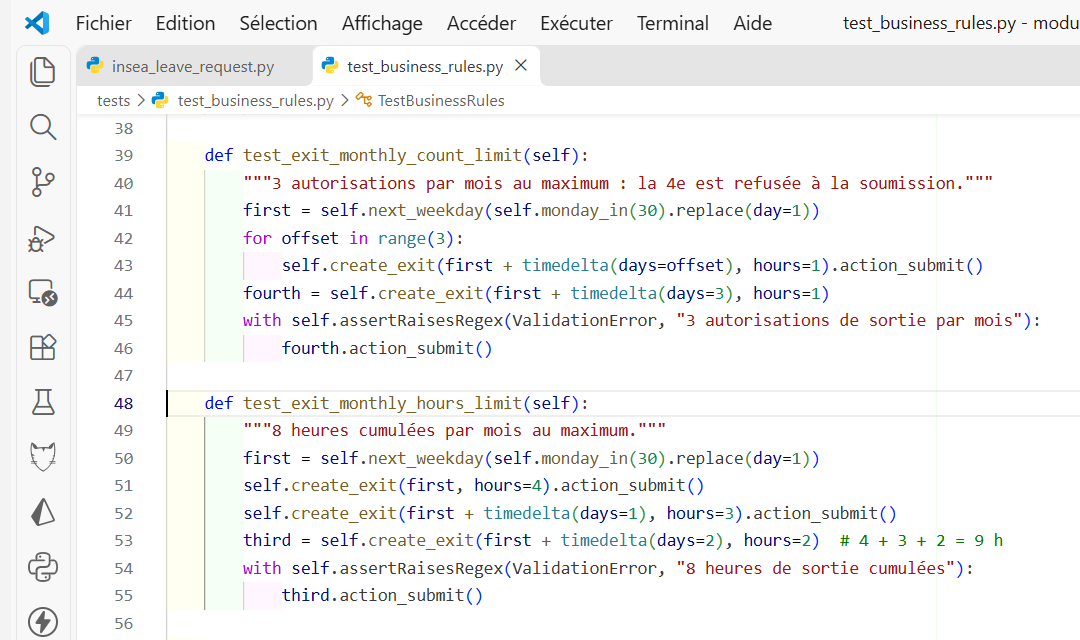
\includegraphics[width=0.86\textwidth]{img/vscode_test.png}
\caption{Deux tests du plafond mensuel des sorties dans \code{tests/test_business_rules.py}
(Visual Studio Code). La 4\textsuperscript{e} sortie du mois, puis une 3\textsuperscript{e} sortie
portant le cumul à 9~h, doivent lever une \code{ValidationError} au message attendu.}
\label{fig:code_test}
\end{figure}

Les tests sont lancés avec le moteur de test d'Odoo :
\begin{lstlisting}[language={}]
odoo -d insea_hr_test -u insea_hr_leave_custom \
     --test-tags /insea_hr_leave_custom --http-port=8099 --stop-after-init
\end{lstlisting}
Résultat obtenu sur Odoo \code{19.0-20261015} :
\begin{lstlisting}[language={}]
odoo.service.server: 49 post-tests in 12.52s, 8722 queries
odoo.tests.result: 0 failed, 0 error(s) of 49 tests when loading database 'insea_hr_test'
\end{lstlisting}

\subsection{Anomalies détectées et corrigées}
Les tests automatisés, puis le déroulement des scénarios de démonstration dans le vrai workflow,
ont révélé plusieurs anomalies que nous avons corrigées :
\begin{table}[H]
\centering
\caption{Anomalies relevées pendant la validation.}
\small
\begin{tabularx}{\textwidth}{Y Y}
\toprule
Constat & Correction \\
\midrule
Un justificatif téléversé par l'employé restait privé : le RH ne le voyait pas et la validation
finale était refusée. & Les fichiers sont rattachés à la demande (\code{res_model},
\code{res_id}) ; leurs droits suivent ceux de la demande. Test dédié ajouté. \\
Le RH ne pouvait pas ouvrir les fiches employés (onglet Congés). & Le groupe RH implique
\code{hr.group_hr_user}. \\
Une sortie de 2~h affichait \og 1 jour \fg{} et un congé de 3~jours \og 57~h \fg{}, ce qui
faussait les totaux. & Une seule unité de durée par catégorie. \\
La liste \og À valider \fg{} d'un manager contenait ses propres demandes. & Ajout de
\code{('user_id', '!=', uid)} au domaine de l'action. \\
Tout utilisateur pouvait remettre en brouillon une demande refusée. & Réservé à l'auteur et au RH. \\
Le compte administrateur recevait toutes les activités RH. & Il n'est sollicité qu'en l'absence de
Responsable RH. \\
\bottomrule
\end{tabularx}
\end{table}

\subsection{Vérifications dans l'interface}
En complément des tests de modèle, l'application a été parcourue dans le navigateur (Chrome
piloté par Playwright) avec trois comptes de démonstration : employé, manager et Responsable RH.
Ce parcours a produit les écrans de la section~\ref{sec:ihm}. Il a vérifié :
\begin{itemize}
  \item les menus et les données visibles selon le rôle ;
  \item le blocage d'une saisie invalide (sortie de 5~h, figure~\ref{fig:err5h}) ;
  \item l'affichage des boutons de validation et de l'assistant de refus ;
  \item l'alerte de justificatif manquant ;
  \item la réception des e-mails dans Mailpit.
\end{itemize}
Il a aussi permis de corriger les défauts d'affichage du tableau précédent. Un guide de recette
manuelle (scénarios employé, manager, RH, circuit complet et sécurité) a été rédigé pour la
démonstration.

\subsection{Jeu de données de démonstration}\label{sec:demo}
Le module fournit la société fictive \og Lambda \fg{} : 9 collaborateurs répartis en 4
départements (Direction Générale, Ressources Humaines, Informatique, Finance), avec un historique
d'acquisition mensuelle depuis janvier. Les 16 demandes sont créées puis déroulées \emph{dans le
vrai workflow}, par l'utilisateur concerné : l'historique, les activités et les e-mails sont donc
authentiques.

\begin{table}[H]
\centering
\caption{Demandes de démonstration par état.}
\small
\begin{tabular}{l c}
\toprule
État & Nombre \\
\midrule
Brouillon & 2 \\
Soumis & 3 \\
Validé manager (dont une sans justificatif) & 2 \\
Approuvé & 7 \\
Refusé (par le manager et par le RH) & 2 \\
\midrule
\textbf{Total} & \textbf{16} \\
\bottomrule
\end{tabular}
\end{table}

Les méthodes \code{insea.leave.demo.load()} et \code{reset()} permettent de charger puis de
réinitialiser ce jeu de données ; les comptes sont listés en annexe.

% =====================================================================
\section{Code source et livrables}\label{sec:depot}
% =====================================================================
L'ensemble du projet est publié dans un dépôt public GitHub :

\begin{center}
\fcolorbox{inseagreen}{inseagreen!6}{%
\begin{minipage}{0.86\textwidth}
\centering\vspace{6pt}
{\small Dépôt du projet}\\[3pt]
{\large\bfseries\href{\repourl}{\nolinkurl{github.com/BassirouKadade/odoo-conges-absences}}}\\[3pt]
{\small Version de référence : \href{\repourl/releases/tag/v1.0.0}{\texttt{v1.0.0}}}
\vspace{6pt}
\end{minipage}}
\end{center}

\begin{table}[H]
\centering
\caption{Contenu du dépôt.}
\small
\begin{tabularx}{\textwidth}{>{\ttfamily}l Y}
\toprule
\normalfont Élément & Contenu \\
\midrule
addons/insea\_hr\_leave\_custom/ & Le module Odoo (modèles, vues, sécurité, données, 49 tests). \\
docker-compose.yml & Pile Docker : Odoo~19, PostgreSQL~16 et Mailpit. \\
config/, .env.example & Modèles de configuration (mots de passe à définir localement). \\
docs/uml/ & Sources PlantUML des diagrammes de la section~\ref{sec:uml}. \\
docs/rapport/ & Ce rapport (PDF), sa source LaTeX et ses illustrations. \\
README.md & Présentation, installation, commandes et démonstration. \\
LICENSE & Licence LGPL-3, déclarée dans le manifeste du module. \\
\bottomrule
\end{tabularx}
\end{table}

Les fichiers contenant des mots de passe (\code{.env}, \code{config/odoo.conf}) sont exclus du suivi
de version ; seuls leurs modèles \code{.example} sont publiés. La version \texttt{v1.0.0} correspond
au code décrit dans ce rapport ; le rapport PDF y est joint. Pour récupérer et lancer le projet :

\begin{lstlisting}[language={}]
git clone https://github.com/BassirouKadade/odoo-conges-absences.git
cd odoo-conges-absences
cp .env.example .env && cp config/odoo.conf.example config/odoo.conf
docker compose up -d
\end{lstlisting}

% =====================================================================
\section{Limites et perspectives}
% =====================================================================
\subsection{Hypothèses et limites connues}
\begin{itemize}
  \item \textbf{Jours ouvrés} : ils sont comptés du lundi au vendredi. Les jours fériés et les
        calendriers de travail d'Odoo ne sont pas pris en compte.
  \item \textbf{Demi-journées} : un congé est compté en jours entiers à partir des dates de début et
        de fin.
  \item \textbf{Acquisition} : le crédit de 1,5~jour s'applique à tout employé actif ; la notion de
        \og travail effectif \fg{} (suspension pendant une absence longue, entrée en cours de mois)
        n'est pas modélisée. Le solde ne connaît ni plafond annuel ni expiration.
  \item \textbf{Validation RH} : elle est exigée pour tous les types de congé, y compris d'une seule
        journée. Le cahier des charges la mentionne pour les congés de plus d'un jour ; ce choix est
        paramétrable par type (\code{requires_hr_validation}).
  \item \textbf{Congé pour décès} : le cahier des charges indique 2 à 3~jours ; nous avons retenu le
        maximum de 3~jours.
  \item \textbf{E-mails} : en démonstration, ils sont capturés par Mailpit. Un déploiement réel
        exigerait un serveur SMTP et la configuration d'un domaine d'envoi.
\end{itemize}

\subsection{Perspectives}
\begin{itemize}
  \item intégrer les calendriers de travail et les jours fériés d'Odoo (\code{resource.calendar}) ;
  \item gérer les demi-journées et une période de référence annuelle pour le solde ;
  \item produire un bulletin PDF de la demande approuvée ;
  \item ajouter des tests d'interface (\emph{tours} Odoo) en complément des tests de modèle.
\end{itemize}

% =====================================================================
\section{Conclusion}
% =====================================================================
Le module \og Congés \& Absences \fg{} répond aux spécifications du mini-projet. Les deux types de
demandes, les règles de gestion et le circuit de validation à deux niveaux sont implémentés et
vérifiés par 49 tests automatisés. Le cloisonnement des données repose sur les mécanismes de
sécurité standard d'Odoo, et l'interface propose les vues demandées : formulaire avec barre de
statut, liste, recherche, calendrier et graphique. La conception UML (cas d'utilisation, classes,
états-transitions, séquence, déploiement) correspond au code livré.

Au-delà du résultat, le projet nous a permis de pratiquer l'intégration d'un besoin métier dans un
ERP : réutiliser l'existant quand il convient (employés, messagerie, sécurité), l'étendre quand il
le faut (\code{hr.employee}) et créer ce qui est propre au métier, en respectant les conventions de
la version~19 d'Odoo.

% =====================================================================
\clearpage
\appendix
\section{Annexes}
% =====================================================================
\subsection{Comptes de démonstration}
Mot de passe commun : \code{lambda2026} (environnement local uniquement).
\begin{table}[H]
\centering
\small
\begin{tabular}{l l l l}
\toprule
Identifiant & Nom & Rôle & Manager \\
\midrule
\code{rachid.elamrani@lambda.ma} & Rachid El Amrani & Directeur Général (manager) & -- \\
\code{salma.bennani@lambda.ma} & Salma Bennani & Responsable RH & Rachid \\
\code{youssef.alaoui@lambda.ma} & Youssef Alaoui & Manager Informatique & Rachid \\
\code{nadia.chraibi@lambda.ma} & Nadia Chraibi & Manager Finance & Rachid \\
\code{karim.idrissi@lambda.ma} & Karim Idrissi & Employé & Youssef \\
\code{imane.tazi@lambda.ma} & Imane Tazi & Employée & Youssef \\
\code{omar.fassi@lambda.ma} & Omar Fassi & Employé & Youssef \\
\code{hajar.berrada@lambda.ma} & Hajar Berrada & Employée & Nadia \\
\code{mehdi.lahlou@lambda.ma} & Mehdi Lahlou & Employé & Nadia \\
\bottomrule
\end{tabular}
\end{table}

\subsection{Mise en route}
\begin{lstlisting}[language={}]
cp .env.example .env
cp config/odoo.conf.example config/odoo.conf     # puis adapter les mots de passe
docker compose up -d                             # Odoo : http://localhost:8070
                                                 # Mailpit : http://localhost:8025
\end{lstlisting}
La base est créée depuis le gestionnaire de bases d'Odoo, puis le module est installé depuis le
menu Applications. Le détail des commandes figure dans le fichier \code{README.md} du projet.

\subsection{Autres écrans}
\fig{img/10_rh_toutes_demandes.png}{Suivi RH : liste de toutes les demandes.}
\fig{img/14_pivot.png}{Tableau croisé : jours par employé et par type.}
\fig{img/19_config_types.png}{Configuration des types de congés.}
\fig{img/23_mailpit_boite.png}{Boîte de réception Mailpit après le chargement de la démonstration.}

\end{document}
